%%%%%%%%%%%%%%%%%%%%%%%%%%%%%%%%%%%%%%%%%%%%%%%%%%%%%%%%%%%%%%%%%%%%
%% I, the copyright holder of this work, release this work into the
%% public domain. This applies worldwide. In some countries this may
%% not be legally possible; if so: I grant anyone the right to use
%% this work for any purpose, without any conditions, unless such
%% conditions are required by law.
%%%%%%%%%%%%%%%%%%%%%%%%%%%%%%%%%%%%%%%%%%%%%%%%%%%%%%%%%%%%%%%%%%%%

\documentclass[
  digital, %% The `digital` option enables the default options for the
           %% digital version of a document. Replace with `printed`
           %% to enable the default options for the printed version
           %% of a document.
%%  color,   %% Uncomment these lines (by removing the %% at the
%%           %% beginning) to use color in the digital version of your
%%           %% document
  table,   %% The `table` option causes the coloring of tables.
           %% Replace with `notable` to restore plain LaTeX tables.
  oneside, %% The `twoside` option enables double-sided typesetting.
           %% Use at least 120 g/m² paper to prevent show-through.
           %% Replace with `oneside` to use one-sided typesetting;
           %% use only if you don’t have access to a double-sided
           %% printer, or if one-sided typesetting is a formal
           %% requirement at your faculty.
  lof,     %% The `lof` option prints the List of Figures. Replace
           %% with `nolof` to hide the List of Figures.
  lot,     %% The `lot` option prints the List of Tables. Replace
           %% with `nolot` to hide the List of Tables.
  %% More options are listed in the user guide at
  %% <http://mirrors.ctan.org/macros/latex/contrib/fithesis/guide/mu/fi.pdf>.
]{fithesis3}
%% The following section sets up the locales used in the thesis.
\usepackage{polyglossia}  %% By using `czech` or `slovak` as the
\setmainlanguage{english} %% main locale instead of `english`, you
%% can typeset the thesis in either Czech or Slovak, respectively.
%% For non-Latin scripts, it may be necessary to load additional fonts:
\newfontfamily\russianfont[Script=Cyrillic,Ligatures=TeX]{PT Serif}
%%
%% The following section sets up the metadata of the thesis.
\thesissetup{
    date        = \the\year/\the\month/\the\day,
    university  = mu,
    faculty     = fi,
    type        = bc,
    author      = Petr Janík,
    gender      = m,
    advisor     = {Ing. Lukáš Grolig},
    title       = {Receipt database with OCR scan},
    % TeXtitle    = {The Proof of $\mathsf{P}=\mathsf{NP}$},
    keywords    = {machine learning, OCR, React Native},
    % TeXkeywords = {keyword1, keyword2, \ldots},
    abstract    = {%
      This is the abstract of my thesis, which can

      span multiple paragraphs.
    },
    thanks      = {%
      I would like to thank my supervisor Ing. Lukáš Grolig for bringing up an incredibly interesting assignment for this thesis. 
      
      Secondly, I would like to acknowledge all my friends, family and colleagues who sent me images of receipts and took part in the survey.
      
      My deepest gratitude belongs to my girlfriend for her endless support, immense encouragement and countless advice.
    },
    bib         = bibliography.bib,
    %% Uncomment the following line (by removing the %% at the
    %% beginning) and replace `assignment.pdf` with the filename
    %% of your scanned thesis assignment.
%%    assignment         = assignment.pdf,
}
\usepackage{makeidx}      %% The `makeidx` package contains
\makeindex                %% helper commands for index typesetting.
%% These additional packages are used within the document:
\usepackage{paralist} %% Compact list environments
\usepackage{amsmath}  %% Mathematics
\usepackage{amsthm}
\usepackage{amsfonts}
\usepackage{url}      %% Hyperlinks
\usepackage{markdown} %% Lightweight markup
\usepackage{tabularx} %% Tables
\usepackage{tabu}
\usepackage{booktabs}
\usepackage{listings} %% Source code highlighting
\lstset{
  basicstyle      = \ttfamily,
  identifierstyle = \color{black},
  keywordstyle    = \color{blue},
  keywordstyle    = {[2]\color{cyan}},
  keywordstyle    = {[3]\color{olive}},
  stringstyle     = \color{teal},
  commentstyle    = \itshape\color{magenta},
  breaklines      = true,
}
\usepackage{floatrow} %% Putting captions above tables
\floatsetup[table]{capposition=top}

% provides subfigure environment
\usepackage{subcaption}

% https://cs.overleaf.com/learn/latex/Code_Highlighting_with_minted
\usepackage{minted}
\usepackage{xcolor}
%\usemintedstyle{manni}
%\definecolor{bg}{rgb}{0.1,0.1,0.1}
\newcommand{\code}[1]{\mintinline[]{javascript}|#1|} % TODO change to jsx and compile locally using 'latexmk -lualatex fi-lualatex.tex' for jsx syntax support (https://tex.stackexchange.com/a/519333)

% Control inline code background dimensions
% https://tex.stackexchange.com/a/276750
% \usepackage{xpatch}

% \newlength{\mintedfboxsep}
% \setlength{\mintedfboxsep}{0.5pt}

% \makeatletter
% \newlength{\fboxrsep}
% \setlength{\fboxrsep}{\fboxsep}

% \newlength{\fboxlsep}
% \setlength{\fboxlsep}{\fboxsep}

% \newlength{\fboxtsep}
% \setlength{\fboxtsep}{\fboxsep}

% \newlength{\fboxbsep}
% \setlength{\fboxbsep}{\mintedfboxsep}

% \xpatchcmd{\minted@inputpyg@inline}{%
%   \colorbox%
% }{%
%   \long\def\color@b@x##1##2##3%
%   {\leavevmode
%     \setbox\z@\hbox{\kern\fboxlsep{\set@color##3}\kern\fboxrsep}%
%     \dimen@\ht\z@\advance\dimen@\fboxtsep\ht\z@\dimen@
%     \dimen@\dp\z@\advance\dimen@\fboxbsep\dp\z@\dimen@
%     {##1{##2\color@block{\wd\z@}{\ht\z@}{\dp\z@}\box\z@}}}%
%   \colorbox%
% }{\typeout{Success}}{\typeout{Failure}}
% \makeatother
% END of 'control inline code background dimensions'

% write thousand comma separator in numbers by wrapping them inside \num{}
% do so also in math mode
% applies only for numbers >= 10,000
\usepackage{siunitx}
\sisetup{group-separator={,}}

% do not wrap equations
\binoppenalty=\maxdimen
\relpenalty=\maxdimen

% add command to create inline color boxes
\makeatletter
\def\testclr#1#{\@testclr{#1}}
\def\@testclr#1#2{{\fboxsep\z@\fbox{\colorbox#1{#2}{\phantom{XX}}}}}
\makeatother

% enables \emoji{} command to insert UNICODE emojis 
% https://mirror.las.iastate.edu/tex-archive/macros/luatex/latex/emoji/emoji-doc.pdf
\usepackage{emoji}

% variables for screen images placed side-by-side
\newcommand\half{0.45}
\newcommand\subfigsize{0.95}

% silence some warnings
\usepackage{silence}
\WarningFilter{biblatex}{File 'american-iso.lbx' not found!}
\WarningFilter{caption}{Cannot determine current font size.}
% c2019 etc. emit warning about not sorting properly, but it is fine, since the entries are processed in citation order - https://www.overleaf.com/learn/latex/Bibliography_management_with_biblatex#Reference_guide
\WarningFilter{latex}{Invalid format}

% add 'L' column type to tabular that aligns text to the left and has fixed width
% https://tex.stackexchange.com/a/12712
\usepackage{array}
\newcolumntype{L}[1]{>{\raggedright\let\newline\\\arraybackslash\hspace{0pt}}m{#1}}
% bigger padding between rows in table
\renewcommand{\arraystretch}{1.5}

% add \Dash command that creates em-dash with thin spaces around
% it can be used as: hello \Dash world (i.e. it will automatically remove surrounding spaces) 
% https://tex.stackexchange.com/a/413058
\DeclareRobustCommand{\thinskip}{\hskip 0.16667em\relax}
\def\emdash{---}
\def\dosh#1#2{\unskip#1\thinskip#2\thinskip\ignorespaces}
\def\Dash{\dosh\nobreak\emdash}
\def\Ldash{\dosh\empty{\hbox{\emdash}\nobreak}}
\def\Rdash{\dosh\nobreak\emdash}

% for defining and introducing new terms
% e.g. \definition{JSON} is a...
\newcommand{\definition}[1]{\textit{#1}}





\begin{document}
\chapter*{Introduction}
\addcontentsline{toc}{chapter}{Introduction}
During everyday life, people take part in transactions. Be it grocery shopping or refuelling of a car. Despite more and more goods being offered online, offline transactions still form an important part of the overall purchases. Proof of such transactions is, in most cases, a receipt. This proof is necessary when complaining or returning goods. However, it can get tough to keep track of all the receipts, and people can be rejected when asking for a refund simply because they either did not keep their receipt or put it among all the other receipts and are unable to find it. The receipt can also get damaged in such a way that it is not readable anymore. 

The goal of my thesis is to develop an application that would serve as a user's digital receipt database. It would allow the user to take a photo of a receipt and by using optical character recognition it would extract the textual information from the photo. This extracted information would be used to pre-fill the receipt record. The receipt records should be editable and searchable, e.g. by the merchant name or items bought. The application should be available on Android and Windows.

In the first chapter, I provide a brief overview of techniques used for data extraction from images.

In the second chapter, I describe currently available applications that are trying to solve this task, their main features and drawbacks.

The next chapter is concerned with choosing the right technology for developing a cross-platform application. This chapter also provides an overview of the chosen framework \Dash React Native.

An essential part of the thesis is testing and continuous integration. The types of testing that were used to ensure the high quality and reliability of the application are described in the fourth chapter.

The fifth chapter describes the functionality of the application. It shows how Microsoft Form Recognizer \cite{WhatIsFormRecognizer} was used to extract the information from a photo of a receipt. This chapter also includes a description of a receipt item categorization using word embeddings. The image processing using the OpenCV\footnote{\url{https://opencv.org/}} library is featured as well.

% compared to other applications
The last chapter provides an evaluation of the application: how well it extracts the data from the photo, how accurate the assigned item categories are and how well it processed the original photo to reduce the noise.

The outcome of the thesis is an application named Receipts Scanner. It can be used as a way to conveniently organize receipts and access them both from mobile and desktop. 

The patterns used in this application can be used for developing other React Native applications. 

\chapter{Existing solutions}

Applications addressing the need for unified digital storage of receipts are usually referred to as expense managers. The most popular expense manager for iOS\footnote{Mobile operating system developed by Apple.} is called Smart Receipts\footnote{\url{https://www.smartreceipts.co/}}. It is also available on Android\footnote{ Mobile operating system developed by Open Handset Alliance and sponsored by Google.}, but it is superseded by an application called Receipt Scanner\footnote{Receipt Scanner on Google Play:\\\url{https://play.google.com/store/apps/details?id=com.easyexpense/}.} in terms of downloads. They allow users to take photos of receipts and fill in additional information such as total price, date of purchase or expense category. These receipts can then be searched by name, price or category. Both applications provide an option to organize expenses into reports. Users can export these reports in CSV format; Smart Receipts also supports PDF export. Another feature is a visualization of expenses throughout time and across categories.

The main feature I will focus on is the automatic information extraction from the receipts. It is available for \$0.1 per scan in Smart Receipts, as of April 2021, and it is free in Receipt Scanner. Other applications that offer this feature are Expensify\footnote{Expensify on App Store:\\\url{https://apps.apple.com/au/app/expensify-receipts-expenses/id471713959}.}, Receipt Lens\footnote{Receipt Lens on App Store:\\\url{https://apps.apple.com/us/app/receipt-lens-receipt-scanner/id1424280764}.} and Dext\footnote{Dext on App Store:\\\url{https://apps.apple.com/us/app/dext-finance-and-accounting/id418327708}.}. All are available for Android and iOS. The amount of information extracted from the picture is, however, limited. Usually, it includes only merchant name, total paid amount, tax amount, date, currency and category. Any information about individual items is missing.

An open-source\footnote{Open-source software is software whose source code is released with permission to use, copy, distribute and modify \cite{GartnerOpenSource}. It is usually free to use. It is often developed collaboratively on platforms such as GitHub.} alternative to the mentioned applications is Receipt Manager\footnote{Receipt Manager on GitHub: \url{https://github.com/ReceiptManager}.}.
It uses Tesseract\footnote{Tesseract is a library and a command line program for extracting textual data from images. Tesseract on GitHub: \url{https://github.com/tesseract-ocr/tesseract}.} for text recognition from the image and a fixed set of rules to extract the information. The main idea of this project is that it does not rely on any third-party services.
It is available on iOS, Android and the Web. All these clients connect to a server on which the data extraction runs. It is deployed separately as a Docker\footnote{TODO} container.

\chapter{Image data extraction}
On a high level, the data extraction from the photo of a receipt involves two steps: optical character recognition and data extraction from text.

\section{Optical character recognition}\index{OCR}
First, the raw textual data need to be extracted. This is done using Optical Character Recognition (OCR). OCR is the process of translating images of handwritten, typewritten, or printed text into a format understood by machines.
It works by pre-processing the image\footnote{Image pre-processing refers to a set of techniques (e.g. noise reduction), that are applied to the image to make it more suitable for the subsequent steps.} and segmenting the text into lines, then words and eventually into individual characters to which a code, such as ASCII, is assigned. \cite{Shreya2019OCRCNN}

The code can be assigned based on template matching. An image of an unknown character is compared to a set of images of known characters. The code of the most similar character is chosen. The similarity can be computed as a difference between the pixel's grayscale value in the unknown character and a pixel's grayscale value in the known character \cite{Ziegaus2016TemplateMatching}.
This approach works well\cite{Ziegaus2016TemplateMatching} for receipts because the characters are printed and are therefore almost the same, except for minor deficiencies in printing. Receipts also usually use the same or a very similar font.

Another approach is to extract the most relevant information from the character image. This is called feature extraction. An example of such a feature could be the density of dark pixels in a given part of the image. These features are used as inputs for machine learning models such as K-Nearest Neighbors and Support Vector Machines. \cite{Singh2011Feature}

The third approach is to use a Convolutional
Neural Network. It has the highest computational cost among the three mentioned approaches and requires a large dataset of images to learn on, but it has the best performance. \cite{Shreya2019OCRCNN}

\section{Data extraction from text}
The second step is to assign a meaning to the parts of the extracted text. This can be done by pattern matching, dictionary matching or using more complex methods such as neural networks. 

Pattern matching uses the fact that some data have a specific format compared to other data available on the receipt. For example, dates and phone numbers can be extracted using regular expressions.

Dictionary matching tries to find a value from a list of possible values. An example would be finding a merchant name in a pre-defined list of merchants.

All methods can take advantage of the actual text position. The merchant name is most likely to appear on the top, the individual items in the middle and the total price at the bottom. However, receipts vary significantly in the locations of different data. Therefore this method, referred to as Zone OCR, is more suitable for forms and invoices where the format is known.

\chapter{Choice of platforms}
\label{chap:choice_of_platforms}
According to Pew Research Center \cite{PewResearchCenter2021Mobile}, as of 2021, 85\% of adults in the United States own a smartphone. There is no dispute about smartphone being a ubiquitous device in people's lives. 
Most smartphones have a decent camera that allows taking photos of receipts in sufficient quality. Therefore most of the focus has been on developing a mobile app.
The next question that needs to be answered is whether to target Android, iOS or both. According to IDC's market research \cite{Idc2021Smartphone}, in 2020, 84.1\% of smartphones were equipped with Android and 15.9\% with iOS. The development of iOS applications requires a Mac\footnote{Mac, also known as Macintosh, is a family of personal computers sold by Apple. Current models include MacBook Pro and iMac.} and Xcode\footnote{Xcode is software by Apple for developing applications for Apple products. See \url{https://developer.apple.com/xcode/}.}. Some workarounds exist around this limitation, but most of them rely on using a Mac in the cloud. At the beginning of the writing of the thesis, I did not have access to Mac. In order to be able to target more devices and given the mentioned limitation, I chose to develop an Android application.

Although smartphones are convenient for taking the photo of the receipt right after the purchase, some users might prefer a desktop application to view and search the receipts.
According to Statcounter \cite{Statcounter2021Desktop}, Windows\footnote{Group of operating systems developed by Microsoft.} operating system makes for 75.55\% of desktop operating systems, macOS\footnote{Desktop operating system developed by Apple.} comes second with 16.5\%\footnote{Data have been collected based on website views.}.
For the same reasons (ability to cover more devices and having Windows PC), I chose Windows as the supported desktop operating system.

\chapter{Choice of technology}
As established in the previous Chapter \ref{chap:choice_of_platforms}, the targeted platforms are Android and Windows. The traditional approach would be to implement a separate application for each platform, for Android using Java or Kotlin, and for Windows using Universal Windows Platform (UWP) or Windows Presentation Foundation (WPF). This approach suffers from the apparent disadvantage of writing the code twice. The functionality of the application differs only slightly on Android and Windows, so the preferred solution is to have a cross-platform application. A cross-platform application is an application that can run on multiple platforms without a need for having a separate code base for each.

There are many available frameworks that aid cross-platform development.

\section{Xamarin}
\textit{``Xamarin is an open-source platform for building modern and performant applications for iOS, Android, and Windows with .NET.''} \cite{WhatIsXamarin} With Xamarin, the business logic and backend code are written in C\# and fully shared.
Xamarin.Forms extends this code reuse to the user interface (UI). The user interface is defined using XAML\footnote{eXtensible Application Markup Language is a markup language based on XML used to define user interfaces \cite{Hermes2019Building}}. It targets iOS, Android, and Windows.

\section{.NET Multi-platform App UI}
.NET MAUI is an evolution of Xamarin.Forms. It targets Android, iOS, Windows and macOS. It is still in a preview version\footnote{Roadmap of.NET MAUI: \url{https://github.com/dotnet/maui/wiki/Roadmap}.}.

\section{Flutter}
\textit{``Flutter is Google’s UI toolkit for building beautiful, natively compiled applications for mobile, web, and desktop from a single codebase.''} \cite{FlutterHomepage} It uses Dart programming language. The desktop support is available as a beta release \cite{FlutterDesktopSupport}.

\section{Capacitor}
Capacitor is an open-source native runtime for building Web Native\footnote{A Web application that accesses native APIs \cite{WebNative}.} apps. It enables development of cross-platform iOS, Android, and Progressive Web Apps \cite{CapacitorHomepage}. Capacitor is developed by Ionic. The application is built using web technologies (JavaScript\footnote{JavaScript is a scripting language targeted specifically to the Internet \cite{GartnerJavaScript}.}, HTML\footnote{Hypertext Markup Language is a document-formatting language used to create Web pages \cite{GartnerHTML}.}, and CSS\footnote{Cascading Style Sheets add style (e.g., fonts, colors, spacing) to Web documents\cite{W3CCSS}.}) and rendered using Web View. Web View resembles a full-screen browser, but it is not limited to browser APIs. It can call native APIs such as sensors and storage.

It is possible to create a desktop application by wrapping the web application inside Electron. Capacitor has built-in support for Electron.

\subsection{Electron}
\label{sec:electron}
Electron is a framework that enables creating desktop applications with JavaScript, HTML, and \textsc{CSS}. These applications can then be run on macOS, Windows, or Linux \cite{WhatIsElectron}. Electron is used, for example, by Visual Studio Code and Slack.

\section{React + PWA + Electron}
React is a JavaScript library for building user interfaces created by Facebook. It is one of the most used libraries for building web applications. It uses JSX, which is a combination of JavaScript and XML\footnote{\definition{Extensible Markup Language} is a W3C open standard for describing data using embedded tags. \cite{GartnerXML}}, for example, \code{const element = <h1>Hello {'react'.toUpperCase()}</h1>;}. React is declarative and component-based, which means that complex UIs are composed of multiple simpler, independent and reusable components. The components are parametrized with properties (very often called \textit{props}).

React itself is not a cross-platform framework. However, if we release the constraint of having a native mobile application, it is possible to create a progressive web application (PWA). Most React starter templates provide this functionality. The PWA looks very similar to the native application. It is installed directly from the browser by visiting the website that provides the PWA. PWA can be installed both on mobile and desktop.
In a similar manner to Capacitor, desktop support is possible by wrapping the React application inside Electron. 

\section{React Native}
React Native is a JavaScript framework created by Facebook. It is based on React, but instead of targeting the browser, it targets mobile platforms \Dash Android and iOS \cite{Eisenman2015Learning}. There are community-supported projects\footnote{\url{https://reactnative.dev/docs/out-of-tree-platforms}} that bring React Native to other platforms, such as React Native Windows, React Native macOS and React Native Web. It is used by companies such as Facebook, Instagram and Shopify. 

Unlike Capacitor, which uses Web Views, React Native is compiled into native code, allowing developers to create applications that look and feel like native applications written in Java/Kotlin (for Android) and Objective-C/Swift (for iOS). It also comes with performance benefits. 

As opposed to React, which uses elements that correspond to HTML elements, e.g. \code{<div>} and \code{<p>}, React Native uses TO platform-agnostic elements such as \code{<View>} and \code{<Text>}. Those are then translated to native UI elements. It also uses its own abstraction of CSS.

React Native exposes JavaScript interfaces for platform APIs so that the applications can access platform features like the camera or the user’s location.

By default, React Native can run on iOS and Android. To run on Windows, React Native Windows is installed into an existing React Native application. After compiling the React Native code, the result will be a UWP application, which can run on Windows PC and other UWP supported devices such as Xbox.

React Native's motto \textit{Learn once, write anywhere.} means that when a developer learns the concepts and syntax of React Native, they should be able to write programs for any platform (that React Native supports). This motto is not to be confused with \textit{Write once, run anywhere.}, which would promise that the same code would be able to run on any platform. However, during the time, and with lots of community efforts, React Native has developed into a framework whose users usually report around 90\% code reuse, which means that only 10\% of code needs to be platform-specific. 

React Native provides easy ways to write platform-specific code that does not affect other platforms. This concept is described in Section \ref{sec:platform_specific_code}.

I chose to develop Receipts Scanner in React Native for its previously mentioned benefits, i.e. native controls, performance, a wide range of supported platforms and also due to my familiarity with React.

\chapter{React Native in detail}

\section{Creating new React Native application}
The official way of creating a new React Native application is to use React Native CLI\footnote{Command Line Interface}. The application produced by the CLI contains only one component. It does not use any additional libraries apart from a linter\footnote{A static analysis tool that highlights errors and enforces good programming practices.} and a testing framework.

Developing applications with React Native is often repetitive, and the same setup needs to be made for every application. To reduce the time it would take to install all required libraries and to enforce the best practices, application boilerplates have been created.

\subsection{Ignite}
The most used boilerplate for React Native is Ignite\footnote{Ignite on GitHub: \url{https://github.com/infinitered/ignite}.}.
Ignite is a CLI and an application boilerplate at the same time. It is opinionated, meaning that it enforces specific project structure and libraries. Navigation, application state management, Storybook component library\footnote{Described in Section \ref{sec:component_library}.}, Detox end-to-end tests\footnote{Described in Section \ref{sec:end_to_end_testing}.} and Reactotron\footnote{Described in Section \ref{phantom:reactotron}.} (for inspecting the application) are already set up. The CLI can be used for generating new components and screens.

\subsection{Expo}
\label{sec:expo}
Expo\footnote{\url{https://docs.expo.io/}} is a framework built on top of React Native. An application created with Expo CLI can run on iOS, Android and the Web. It provides many external tools that help with the development process. 
Many libraries for React Native have been created by Expo. Those libraries can be often used also in applications that do not run on Expo.

It is not possible to add a React Native for Windows to the Expo project. For this reason, Receipts Scanner was set up with the React Native CLI instead.

Expo will likely support React Native for Windows in the future\footnote{Feature request to support React Native for Windows in Expo: \url{https://expo.canny.io/feature-requests/p/support-for-react-native-windows-apps}.}.

In the meantime, the Expo built for the Web could be run on Windows using Electron\footnote{Expo has been introduced in Section \ref{sec:electron}.}.

\section{Native Modules}
Native modules provide access to the native platform API that is not available by default in JavaScript \cite{RNNativeModulesIntro}, for example, an API to select a picture on the device. Other reasons for using native modules are taking advantage of existing native libraries or running multi-threaded code.

Native modules for Android are written in Java or Kotlin.
For Windows, they can be written in C++ or C\#, but C++ is the preferred language, primarily due to its performance.

Native modules can be written directly in the application or added as an external package. React Native Directory\footnote{\url{https://reactnative.directory/}} provides a list of available native modules. They can be filtered by the supported platform because the native module is often unavailable on all platforms that React Native supports.

In my opinion, not having a native module's functionality available for a given platform is the most considerable drawback of using React Native.
Most native modules are made for Android and iOS only and cannot be therefore used on the Web or Windows. The missing Windows support is an obstacle encountered many times during Receipts Scanner development.

In case a native module is not available on a given platform, there are four available options:
\begin{enumerate}
    \item \textbf{Omitting the module.} 
    
    If the functionality provided by the native module is not critical, it might be omitted on a given platform. This is possible by having a different code for each platform. This concept is described in Section \ref{sec:platform_specific_code}.
    
    In Receipts Scanner, this approach has been taken with Google Sign In\footnote{Authentication using Google, further described in Section \ref{phantom:google_sign_in}.}, which is not available on Windows.
    
    \item \textbf{Mocking the module.}
    
    In the context of this thesis, \textit{mocking}\index{mocking} means substituting an object or a whole module with a simpler implementation. The simpler object is called a \textit{mock}.
    
    The approach of mocking a module has been applied in Receipts Scanner on NetInfo module, which provides information about the internet connection. Currently, it is not possible to use NetInfo on Windows\footnote{GitHub issue: \url{https://github.com/react-native-netinfo/react-native-netinfo/issues/306}.}. Therefore it has been temporarily mocked always to return information about the device being online.
    
    \item \textbf{Replacing the module.} 
    
    In case a different module that provides similar functionality is available, it can be used instead. If such a module does not exist, it can be implemented.
    
    Receipts Scanner implements its own\footnote{FilePicker} module to provide the functionality of picking an image from the file system on Windows.
    
    \item \textbf{Adding the missing platform to the module.}
    
    Most of the modules are open-source projects to which anyone can contribute. React Native is a relatively new ecosystem and relies on community contributions. In general, anyone can add a new platform to an existing library.
\end{enumerate}

\section{Platform-specific code}
\label{sec:platform_specific_code}
Sometimes it is necessary to have a different code for a different platform. The main reasons are:
\begin{itemize}
\item some platform does not support certain functionality, or the same functionality needs to be implemented differently,
\item the application on a particular platform should behave differently,
\item the styles need to be different.
\end{itemize}

React Native provides two ways of separating code by platform:
\begin{enumerate}
\item \textbf{\texttt{Platform} module}
    
    By writing \code{Platform.OS === 'windows'}, it is possible to determine if the code is running on Windows.
\item \textbf{Platform-specific file extensions}

    If there are two files, \texttt{Button.android.ts} and \texttt{Button.windows.ts} and the \texttt{Button} is imported as \code{import Button from './Button';}‚ the file with the extension of the platform on which the application is running will be picked.
\end{enumerate}

In Receipts Scanner, the \texttt{Platform} module's functionality is used, for example, in the following places:
\begin{itemize}
    \item to allow scanning of a receipt only on Android,
    \item to use different styles for each platform,
    \item to use Google Sign In only on Android,
    \item in Firebase adapter\footnote{Described in Section \ref{phantom:firebase_adapter}.} to use a different Firebase library for each platform,
    \item to use a different \texttt{Modal}\footnote{A component that appears on top overlaying other components. The background is usually grayed out.} component for each platform.
\end{itemize}
Most of these were driven by libraries not having support for React Native Windows.

\chapter{Development}
\section{Version control system commit messages}
When working with a version control system\footnote{Software for tracking changes in files, for example, Git.}, it is good to indicate the type of source code change in a commit message. This can be done either verbally or using an emoji.
Using emojis in commit messages provides an easy way of identifying the purpose or intention of a commit. In the Receipts Scanner repository, the notation in Figure \ref{fig:emoji_commits} has been used. It is loosely based on Gitmoji\footnote{Gitmoji is an initiative to standardize and explain the use of emojis on GitHub commit messages. See \url{https://gitmoji.dev/}.}. The Figure \ref{fig:emoji_commits} shows a Unicode\footnote{\textit{``The standard for digital representation of the characters used in writing all of the world's languages.''} \cite{Unicode}} representation of an emoji and its meaning.

\section{Component library}
\label{sec:component_library}
When developing a React application, it is a good practice to have a set of basic components from which more complex ones are built up. The set of those foundational components is called a component library or a design system. An efficient way of building the component library is by using a tool that allows the development of each component in isolation. 

Storybook\footnote{\url{https://storybook.js.org/}} is a widely used tool for developing UI components in isolation. It is based on plugins. Thanks to its open-source nature, there are many plugins created by the community, which extend the core functionality of Storybook.

Storybook is based on the concept of stories. A story is a permutation of the component with given properties. Each component can have multiple stories. A \texttt{Button} component could have one story displaying the Button in its \textit{enabled} state and a second one for the \textit{disabled} state.

Storybook stories serve as a gallery of available components and as a documentation of their properties. They can be used for snapshot and visual tests, which are described in Sections \ref{sec:snapshot_testing} and \ref{sec:visual_testing} respectively.

Storybook supports multiple platforms, including React and React Native. To better distinguish between the two, I will refer to Storybook for React as \textit{Storybook for Web} because React is a web framework.

Whereas Storybook for Web runs in a web browser, Storybook for React Native needs to run on a mobile device because React Native uses native components that cannot be displayed in the browser.

\phantomsection
\label{phantom:reactotron}
Running Storybook on a mobile device is achieved by rendering the Storybook component instead of the root component that would normally be rendered. To not have to replace the component manually in code every time, Receipts Scanner takes advantage of Reactotron\footnote{Reactotron on GitHub: \url{https://github.com/infinitered/reactotron}.}. Reactotron is a desktop application that provides a suite of tools for easier development in React Native. It is integrated inside the project, so it is possible to switch between displaying Storybook and the actual application from the Reactotron UI. 

Figure \ref{fig:storybook_rn} shows the component library and the interface of Storybook for React Native.

\begin{figure}
    \centering
    \begin{subfigure}[t]{\half\textwidth}
      \centering
      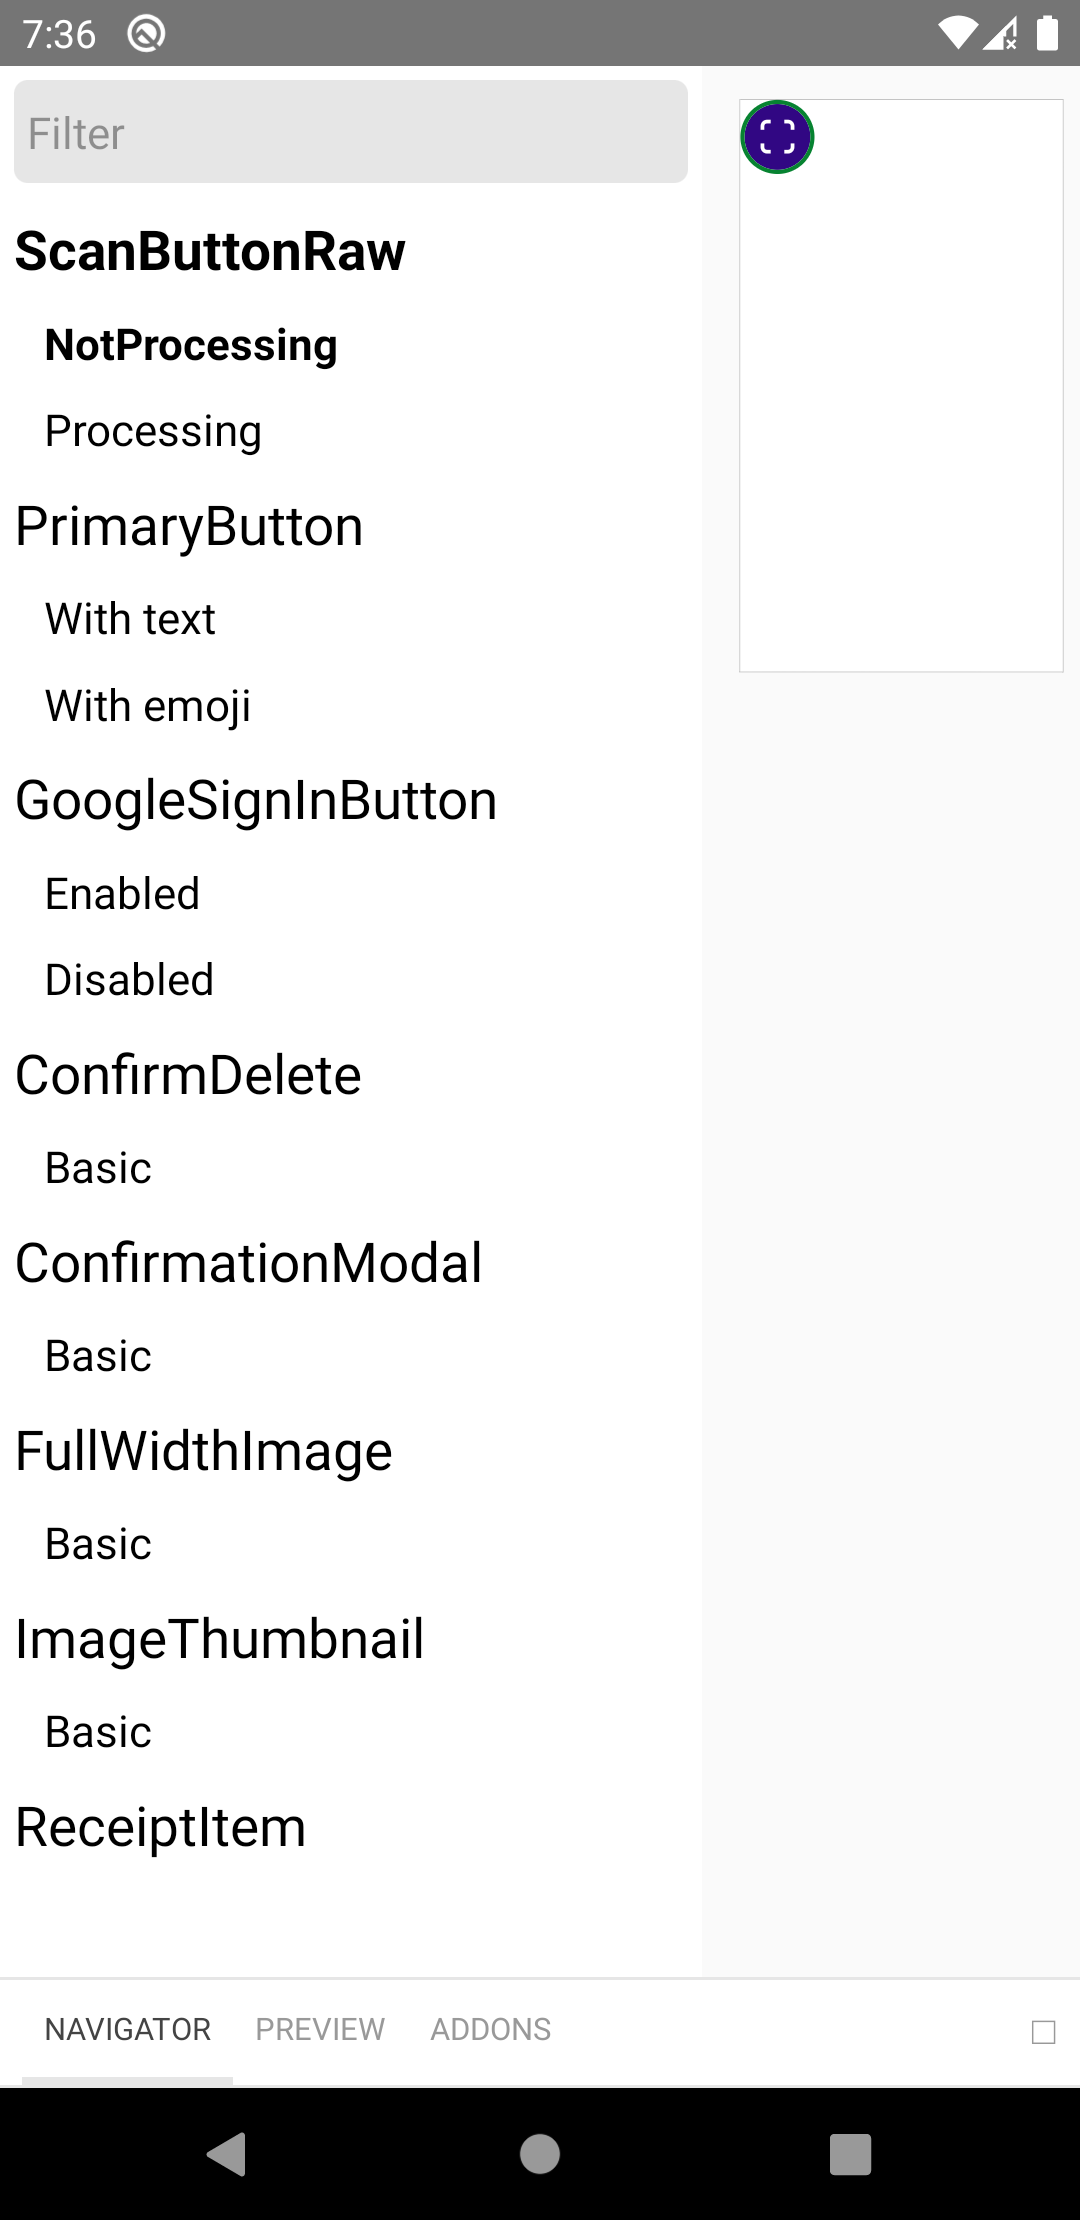
\includegraphics[width=\subfigsize\textwidth]{figures/other/storybook_rn_menu}
      \caption{Menu of components.}
      \label{fig:storybook_rn_menu}
    \end{subfigure}
    \begin{subfigure}[t]{\half\textwidth}
      \centering
      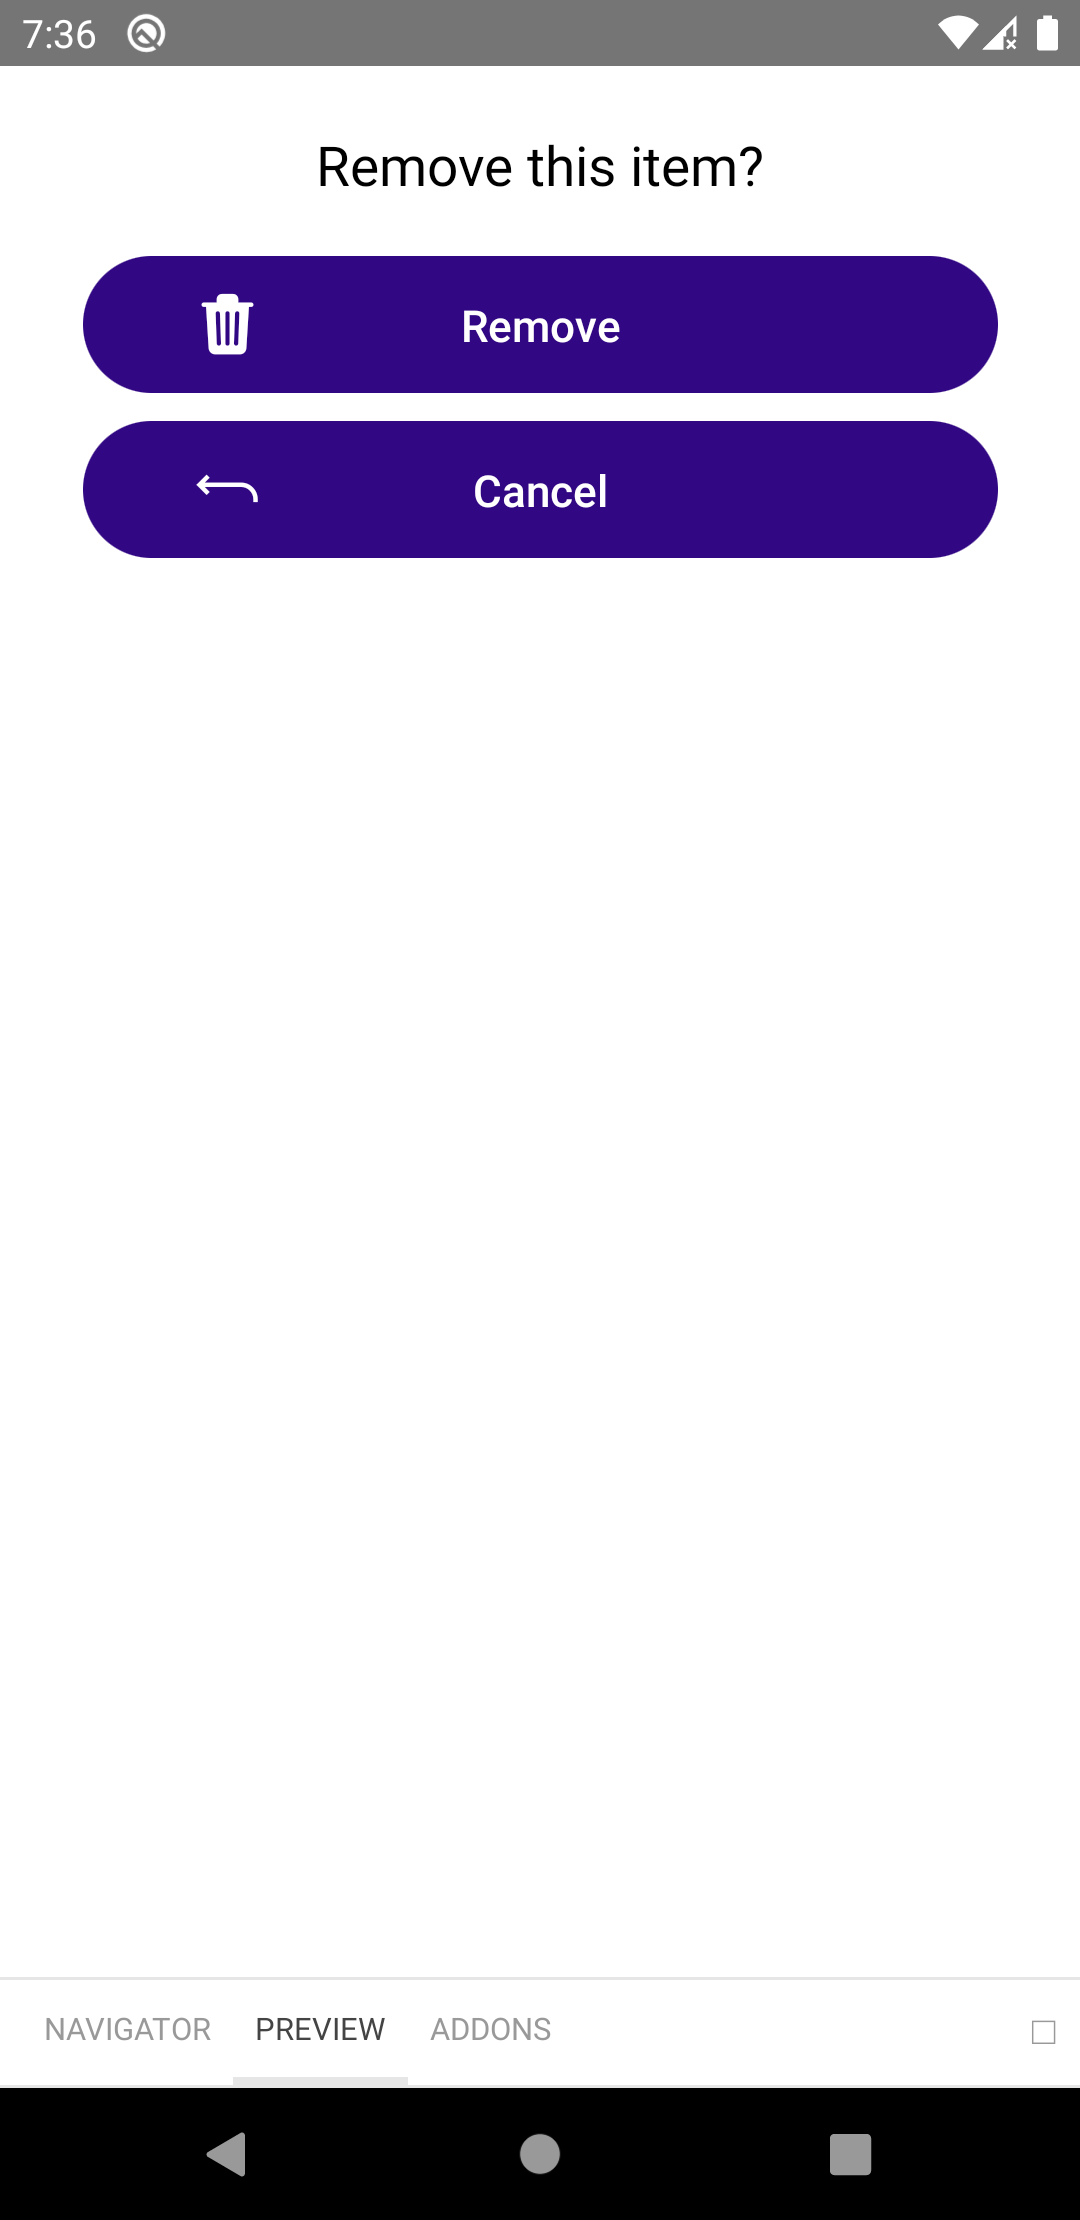
\includegraphics[width=\subfigsize\textwidth]{figures/other/storybook_rn_confirm_delete_component}
      \caption{Detail of \textit{Confirmation Dialog} component.}
      \label{fig:storybook_rn_confirm_delete_component}
    \end{subfigure}
    \caption{Storybook for React Native.}
    \label{fig:storybook_rn}
\end{figure}

It is possible to install a Storybook server that enables navigation between stories directly in the browser. However, the stories are still displayed only on mobile device. In order to show the stories in the browser, a react-native-web\footnote{\url{https://necolas.github.io/react-native-web/}} library must be used. This library provides the same elementary components that are used to create React Native applications. The difference is that instead of translating those components into Android and iOS native components, it translates them into HTML elements.

\begin{enumerate}
    \item \textbf{Adding Web support to the whole application.}
    
    All react-native components are replaced by react-native-web components by aliasing react-native imports to react-native-web in the bundling\footnote{Bundling is the process of transpiling all source files and assets of the application, usually into one large JavaScript file that can be run across different browsers.} process of the whole application. This makes the whole application run in the browser. The Storybook functionality is, therefore, a side-effect.
    
    The Expo\footnote{Expo has been introduced in Section\ref{sec:expo}.} applications can run in the browser by default. They are set up with react-native-web from the beginning. No extra configuration is necessary to have Storybook for React Native running in the browser.
    
    \item \textbf{Installing Storybook for Web.} 
    
    It is possible to install Storybook for Web and alias react-native imports to react-native-web in the bundling process of Storybook. This approach is used in Receipts Scanner. Figure \ref{fig:storybook_web} shows the component library and the user interface of Storybook for Web.
    
    An advantage of this approach is that even though Storybook for React Native is in version 5, the Storybook for Web can use the latest version 6 (as of May 2021). In version 6, all stories in the projects are found automatically without having to list each story explicitly. It also uses a more concise and more intuitive syntax for writing stories.
    
    Another advantage is that the Storybook for Web can be used with other libraries for web development, such as Chromatic for visual testing, which is described in Section \ref{sec:visual_testing}. Storybook for Web can be built into static files and served as an application independent of the React Native application.
    
    The main disadvantage is that there are two separate Storybooks in the project. A small amount of extra code needs to be written for each story to make it visible in both Storybooks. 
    
\end{enumerate}

\begin{figure}
    \begin{center}
        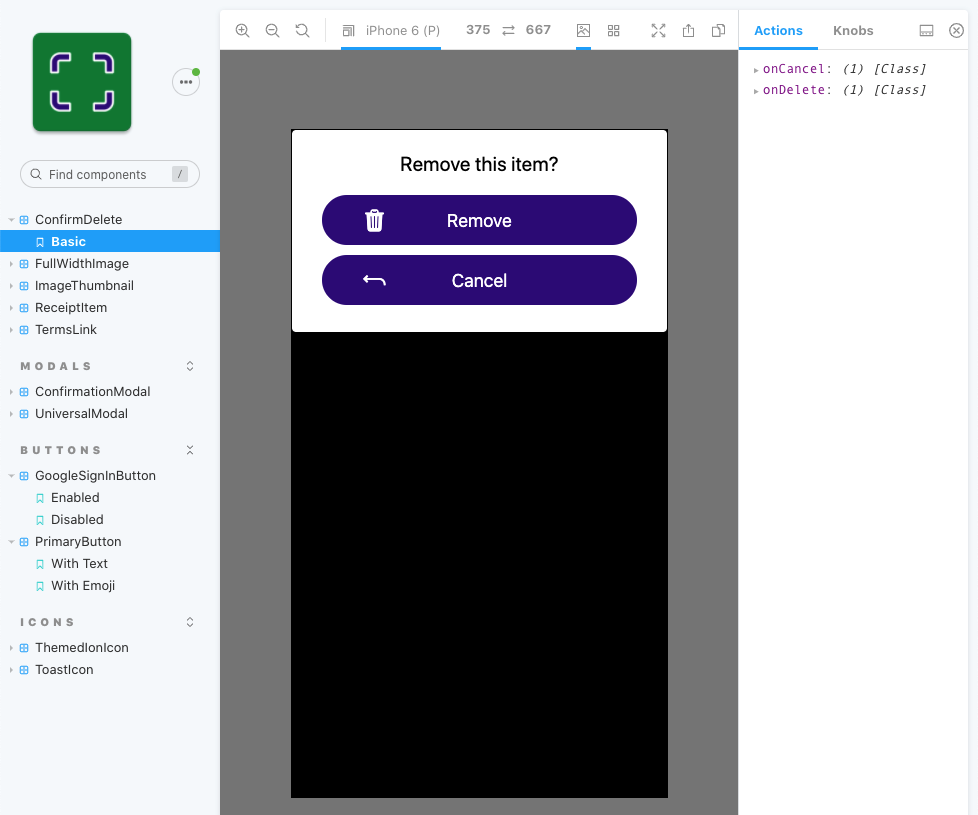
\includegraphics[width=\textwidth]{figures/other/storybook_web}
    \end{center}
    \caption{Storybook for Web in the browser.}
    \label{fig:storybook_web}
\end{figure}

\section{Logging}
The logging in Receipts Scanner happens via methods of a \texttt{LOG} object. This abstraction ensures that the application does not depend on a particular logging system.

All logs are sent to the console in development mode. \texttt{WARN} and \texttt{ERROR} level messages are sent into Sentry\footnote{\url{https://sentry.io/}}, both in development and release mode. Sentry is a third party service that collects logs, errors, and events sent through the network. This enables monitoring of the application behaviour on users' devices.

\section{Testing}
The Receipts Scanner uses five types of tests: unit tests, component tests, snapshot tests, visual regression tests and end-to-end tests.
Apart from visual tests, all tests use a JavaScript testing framework Jest\footnote{\url{https://jestjs.io/}} that is included by default in new React Native applications. The tests run in a Node.js\footnote{Node.js is a JavaScript runtime. See \url{https://nodejs.org/}.} environment that mimics the environment of a React Native application. 

\subsection{Unit tests}
Unit tests cover a single piece of functionality, usually individual functions. In Receipts Scanner, their main goal is to assure that the utility functions such as RGB to HEX color conversion or receipt filtering work.

\subsubsection{Mocking}
When the tested function or object has any dependencies, they are often mocked out.

\subsection{Component tests}
Component tests test individual React components. An example could be a test for a \textit{Receipts List} component. Let us assume that the component calls an API and displays the returned receipts. The test would mock the API call by returning a fixed list of receipts and then assert that those receipts are visible. 

In React Native, there is an option to choose between two libraries for component tests: react-test-renderer and React Native Testing Library. 

react-test-renderer renders components to pure JavaScript objects without depending on the DOM\footnote{Document Object Model} or a native mobile environment \cite{ReactTestRenderer}. It provides methods for locating elements, for example, by component type (e.g. \texttt{Text}) or properties (e.g. finding a button with \texttt{title} value equal to \textit{Submit}).

It is possible to get the rendered component as a JSON\footnote{JavaScript Object Notation is a lightweight data-interchange format \cite{Ecma2017JSON}.} and use it for snapshot testing. Snapshot testing is described in Section \ref{sec:snapshot_testing}.

The issue of testing with react-test-renderer is that the tests rely on implementation details of the components. React Native Testing Library solves this problem by providing utility functions on top of react-test-renderer \cite{ReactNativeTestingLibrary} for locating elements, e.g. by the visible text or accessibility label so that tests resemble how users interact with the application. It is inspired by React Testing Library \cite{ReactNativeTestingLibrary}, which is a widely used testing library for React.

React Native Testing Library also adds a \texttt{fireEvent} method that can simulate \textit{press}, \textit{scroll} and \textit{text changed} events. Therefore both the rendering of the element and interaction with it can be tested.

\subsubsection{Mocking}
Because the components are rendered with react-test-renderer into pure JavaScript objects without depending on a native mobile environment, any native modules need to be mocked.

\subsection{Snapshot testing}
\label{sec:snapshot_testing}
Snapshot tests verify that the rendered markup of the components stays the same. When the snapshot tests are run for the first time, the rendered markup is saved in a file.
During subsequent runs, the newly rendered markup is compared to the saved one. The tests fail when there are differences between the two. Those differences are usually highlighted for the developer to assess whether or not this change was intentional. If it was, the saved snapshots are updated. Otherwise, the unintentional changes are fixed.

It is possible to create snapshot tests with Jest and react-test-renderer by rendering the component to JSON and comparing it to the previously rendered version\footnote{See snapshot testing with Jest: \url{https://jestjs.io/docs/snapshot-testing}.}. This process can be automated with Storybook. Using a Storybook addon StoryShots\footnote{\url{https://www.npmjs.com/package/@storybook/addon-storyshots}}, all stories in the project are turned into snapshot tests. This is a very efficient and inexpensive way of testing because the stories most of the time already exist.

Snapshot testing catches only changes in markup. If, for example, an image on a given URL changes, the snapshot tests will still pass. 

On the other hand, changing markup does not necessarily mean that the result is different. It is often the case that even though the markup has changed, the page looks the same as before, and the tests report false positives. It can be hard to tell whether the change is intended, especially when dealing with large snapshots.

\subsubsection{Mocking}
Because the StoryShots addon uses react-test-renderer internally to render the components and save their snapshot, any native modules need to be mocked.

\subsection{Visual testing}
\label{sec:visual_testing}
Visual testing addresses the issues of snapshot testing mentioned earlier. It is not crucial if the markup changed. The important thing is whether the component looks as desired. Visual tests, also called visual regression tests, assure that once the expected look of a component was achieved, it will stay unchanged.

Visual testing compares screenshots of newly rendered components with the old screenshots, also called reference images.
When visual tests run for the first time, a set of screenshots is made. During subsequent runs, those screenshots are compared to the stored ones. Possible differences are highlighted. There are various tools that can highlight the differences between images. Those tools can be independent of tools used to take the screenshots.

A widely used tool for visual testing in React community is Chromatic\footnote{See \url{https://www.chromatic.com/}.}. It creates screenshots of the Storybook stories. It is not possible to use Chromatic with Storybook for React Native. Receipts Scanner repository uses Storybook for Web too by utilizing react-native-web. The Chromatic is therefore set up for testing components with Storybook for Web.

Chromatic runs in the continuous integration (CI) pipeline\footnote{A series of steps executed when changes are pushed to the remote project repository. Described in Section \ref{sec:continuous_integration}.}. The changes need to be reviewed on the Chromatic website created for the given CI run. Chromatic also publishes the Storybook as a website.

Figure \ref{fig:chromatic_diff} shows how the review process of a visual change in Chromatic UI looks. Both the visual change and the change in the markup are visible.

\begin{figure}
    \begin{center}
        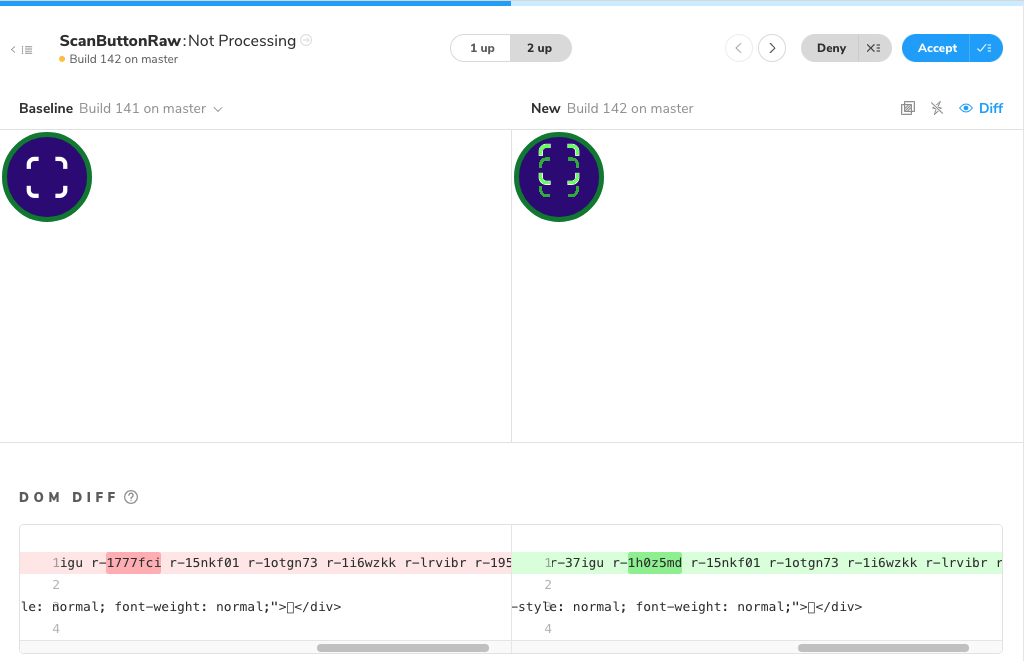
\includegraphics[width=\textwidth]{figures/other/chromatic_diff}
    \end{center}
    \caption{Chromatic screen for reviewing visual change of the \texttt{ScanButtonRaw} component. The Scan icon moved up.}
    \label{fig:chromatic_diff}
\end{figure}

An alternative to Chromatic is a tool called Loki\footnote{\url{https://loki.js.org/}}, which also integrates with Storybook. It can take screenshots in a Chrome browser, on an iOS simulator or on an Android emulator, which means that it can be used both with Storybook for Web and Storybook for React Native.

Loki creates images that highlight the visual change. A visual change of a \textit{Scan Button} component is shown in Figure \ref{fig:loki_diff}.

\begin{figure}
    \begin{center}
        
\includegraphics[width=0.3\textwidth]{figures/other/loki_diff}
    \end{center}
    \caption{Image generated by Loki indicating a visual change to the \texttt{ScanButtonRaw} component. The Scan icon moved up.}
    \label{fig:loki_diff}
\end{figure}

I would not recommend using Loki for Storybook for React Native. The tests are unstable, and the screenshots differ even though the component itself has not changed. This is caused by the component not being fully loaded when the screenshot is made. Loki uses a running Storybook server for controlling which story is shown, which sometimes does not work, resulting in flashing between different stories.
Loki performs better with Storybook for Web, but it cannot take screenshots of modal components.

The third approach of visual testing I tried was a combination of Storycap\footnote{Storycap on GitHub: \url{https://github.com/reg-viz/storycap}.} and Reg Suit\footnote{Reg Suit on GitHub: \url{https://github.com/reg-viz/reg-suit}.}. Similar to Chromatic, Storycap and Reg Suit work only with Storybook for Web.

First, Storycap takes screenshots of the stories. Reg Suit then downloads the previous screenshots from Google Cloud Storage, compares them with the new ones and stores the differences. 

Storycap and Reg Suit should run in the CI pipeline. From my experience, Reg Suit had issues determining the hash of the previous commit. This hash is used to pick correct images from the Google Cloud Storage bucket for comparison. For this reason, all stories were being reported as new, and no comparison took place.

Naturally, it is not good to use all three solutions for visual testing together. I would suggest using only Chromatic because it has a fast setup, provides a clean user interface for reviewing the changes, and seems the most reliable solution among those I have tried.

Similarly to snapshot tests, the visual tests are created automatically from stories. The visual testing is therefore very convenient.

\subsubsection{Mocking}
Visual tests require Storybook to be running. If the Storybook is running on an Android device, no mocking is necessary. If Storybook for Web is used, native modules that do not have web support need to be mocked.

The need for mocking can be alleviated by separating the view part of the application from the business logic.
The components can be divided into two categories: pure and connected. Pure components are components that display data based on their properties. Connected components connect to the database, make API calls and depend on native modules. They pass the data to pure components. In general, stories are written for pure components. Therefore no mocking of native modules is needed.

\subsection{End-to-end testing}
\label{sec:end_to_end_testing}
End-to-end tests are used to test user interaction with the application from the beginning to the end. 

An example of an end-to-end test would be testing the sign-in functionality, i.e. after the required fields of the sign-in form are filled in, and the \textit{Sign in} button is pressed, a screen for the authenticated users is shown.

Multiple end-to-end testing frameworks for React Native exist. Receipts Scanner uses Detox\footnote{Detox on GitHub: \url{https://github.com/wix/Detox}.} end-to-end tests. Detox is a popular choice for React Native testing, mostly for its speed and reliability. Apart from test logs, it can capture screenshots and videos of the running tests, providing greater insight into why tests are failing.

A more recent project, Cavy\footnote{\url{https://cavy.app/}}, takes a different approach from Detox. It does not use any native code. All functionality is achieved with pure JavaScript. The setup is, therefore, more straightforward, but the functionality is limited.

Whereas Detox can locate elements by text or label, Cavy needs each component that is being tested to be wrapped with a special function. This creates noise in the code

The oldest testing framework of the ones mentioned is Appium\footnote{\url{http://appium.io/}}. Similar to Selenium WebDriver\footnote{Selenium is software for automated testing of web applications.}, it uses WebDriver protocol\footnote{WebDriver protocol is used to control the browser.}. It could be used for testing both the Android and the Windows version of Receipts Scanner.

Appium tests are referred to as \textit{black-box} tests. Black-box testing ignores the internal mechanism of a system and focuses solely on the outputs generated in response to selected inputs and execution conditions \cite{Gao2003Testing}. In practise this means, that when a certain element is expected to be visible, Appium polls until the element becomes visible or until a timeout occurs. This usually leads to flaky and non-deterministic tests.

Detox has been created to address this issue. Detox tests are so-called \textit{gray-box} tests, which means that the tests are aware of the internal state of the application. Detox automatically waits until all asynchronous operations (such as querying a server or animations) end, and only then is the assertion triggered.

\subsubsection{Mocking}
Because the Detox tests run on the device (Android or iOS), the native modules need not be mocked. It is still possible to mock external dependencies to make the tests faster and more stable.

\section{Continuous integration}
\label{sec:continuous_integration}
Continuous integration is a practise of frequently merging code changes into a central repository. The changes are validated by creating a build and running automated tests. \cite{Fowler2006Continuous}

Receipts scanner takes advantage of GitHub Actions\footnote{\url{https://github.com/features/actions}}. Every time new code is pushed to the main branch of the GitHub repository, three workflows are run. A workflow consists of multiple jobs that run in parallel. Each job consists of multiple sequential steps.

During the first workflow,
\begin{itemize}
    \item the code is checked for any linting or type errors,
    \item a suite of unit and snapshot tests runs,
    \item Storybook is deployed and visual tests run,
    \item a release version of Android application is built,
    \item a release version of Windows application is built.
\end{itemize}

The second workflow runs end-to-end tests on an emulated Android device.

The third workflow runs tests of the Python API\footnote{Python API is described in Section \ref{sec:python_api}.}. The workflows do not contain the Python API deployment logic. Instead, a repository hook is set up in the Google Cloud Platform Console\footnote{A user interface to manage services provided by Google.} to deploy the latest version of the Python API.

\chapter{Implementation}

\section{Storage}
\label{sec:storage}
The Receipt Scanner needs to store two kinds of data: textual data, i.e. data about the receipts and the users' credentials, and the receipt images.

\subsection{Textual data}
For textual receipt information, document-oriented databases are a perfect fit because they make it easy to store data in the same format and shape as they are used in the application. 
All data of a given object (for example, receipt) can be stored in one document. The documents are stored mostly in JSON, BSON\footnote{Binary JSON.}, XML or YAML\footnote{\definition{YAML} is a human-readable data-serialization language.} format. Unlike SQL databases, document-orient databases do not have a schema and are therefore more flexible.

The documents are stored in collections. Documents can also contain subcollections of documents.

Two very popular document-oriented databases are MongoDB\footnote{\url{https://www.mongodb.com/}} and Google Firestore\footnote{\url{https://firebase.google.com/products/firestore}}. MongoDB uses BSON to store documents, Firestore uses JSON. Both databases support data types such as strings, numbers, arrays and timestamps\footnote{Supported data types in MongoDB: \url{https://docs.mongodb.com/manual/reference/bson-types/}.
Supported data types in Google Firestore: \url{https://firebase.google.com/docs/firestore/manage-data/data-types}.}.

Although document-oriented databases do not have a schema, it is beneficial to have a fixed data model so that the shape of the stored data is predictable.
The data model for Receipts Scanner is shown in Figure \ref{fig:data_model_firestore}. It shows how the data are structured into two collections, \texttt{Users} and \texttt{Receipts}. Because all user data are child nodes of a given user document, it is easy to restrict access to other documents based on the path to that document. The authentication and access rules are described in Section \ref{ref:authentication}.

Although the item forms a separate entity, it is not a document but only an object in the array of items of the receipt.

Other notable fields are \texttt{urlOriginal} and \texttt{urlProcessed}, which specify the URL address of the original receipt photo and a processed photo, respectively. 

    \begin{figure}
        \begin{center}
            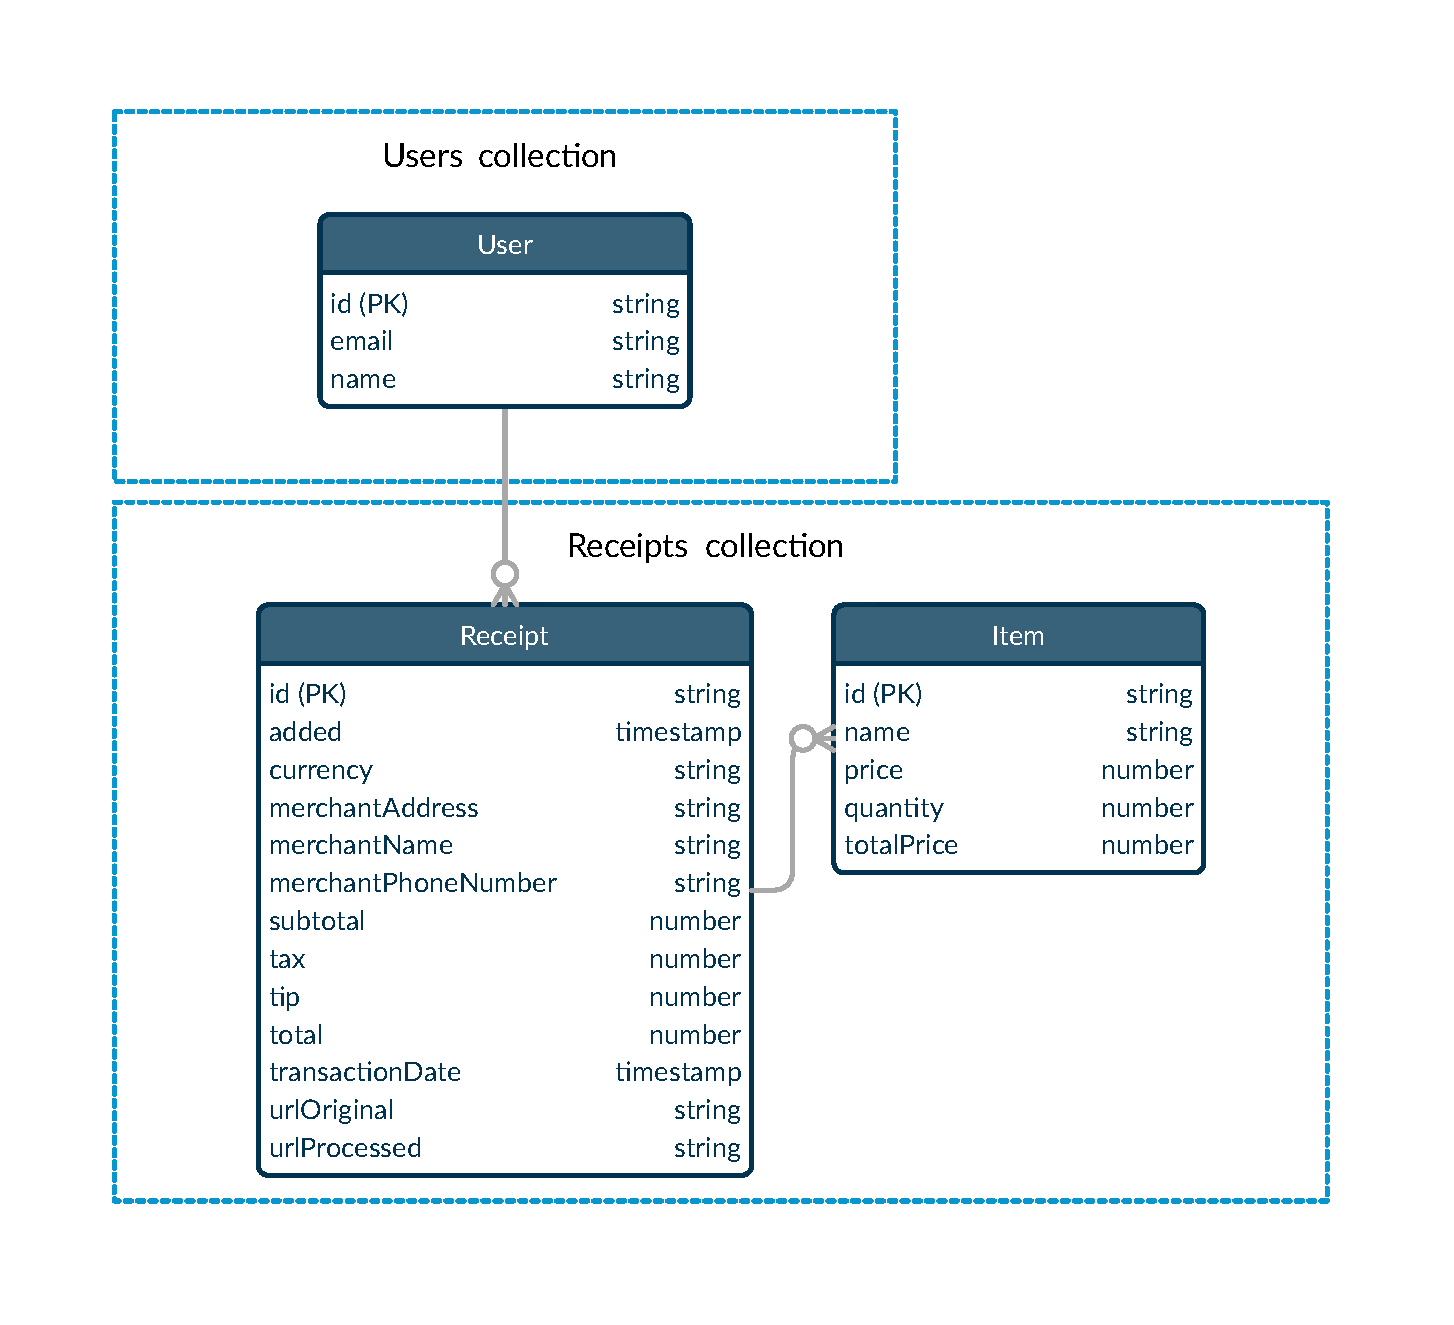
\includegraphics[width=\textwidth]{figures/other/data_model_firestore}
        \end{center}
        \caption{Data model of Receipts Scanner}
        \label{fig:data_model_firestore}
    \end{figure}

\subsection{Image data}
Although storing images directly in the document-oriented database would be possible\footnote{In MongoDB, it is possible to store BSON documents up to 16 MB. Larger files can be split into parts of 255 kB using GridFS \cite{GridFS}}, this solution is not optimal.

For receipt images, the most cost-effective storage is object storage. \definition{Object storage} is storage optimized for storing BLOBs (Binary Large Objects). BLOB is a collection of binary data stored as a single entity. It can be, for example, an image, audio or video. 

The images are stored inside \texttt{Users/<user\_id>/Receipts/} directory. This folder structure enables restricting access to images based on the value of \texttt{<user\_id>}.

I have chosen Google Firestore to store the textual data and Google Storage to store the photos of receipts. These two cloud-based services are available under a platform called Firebase. The Firebase platform also provides authentication and analytics services to Receipts Scanner.

\phantomsection
\label{phantom:firebase_adapter}
Firebase is supported on iOS, Android and the Web. An unofficial library named React Native Firebase\footnote{\url{https://rnfirebase.io/}} provides the same services on React Native for Android and iOS. However, it does not support React Native Windows. Therefore Receipts Scanner uses Firebase for Web on Windows and React Native Firebase on Android. To be able to write the same code that could be run both on Android and Windows, an adapter \texttt{firebase.ts} was created. It imports both libraries, and, based on the platform the application is currently running on, it exports the proper objects. The rest of the code that needs to work with Firebase imports the objects from \texttt{firebase.ts} instead of importing them directly from Firebase for Web or React Native Firebase.

In theory, the Receipts Scanner could use Firebase for Web both on Android and Windows, but I would expect React Native Firebase to be more suitable and faster since it uses native APIs. React Native Firebase could also get support for React Native Windows in the future.

\section{Authentication}
\label{ref:authentication}
\textit{"Authentication is the process of verifying an entity’s identity, given its credentials."} \cite{Cankaya2011Authentication} In Receipts Scanner, users are being authenticated.

The authentication in the application serves two purposes. The first one is the ability to connect saved receipts with the user who created them. The second reason for authentication is to ensure proper database rules. The rules are set so that only authenticated user can create a new \textit{User} document\footnote{Documents and data model of Receipts Scanner have been introduced in Section \ref{sec:storage}.}. The user can read and modify the \textit{User} document if they are authenticated and if the document belongs to them. The last rule ensures that each user can create, read and modify only their receipts inside the \textit{Receipts} collection and not receipts of other users.

\begin{figure}
\centering
\begin{subfigure}[t]{\half\textwidth}
  \centering
  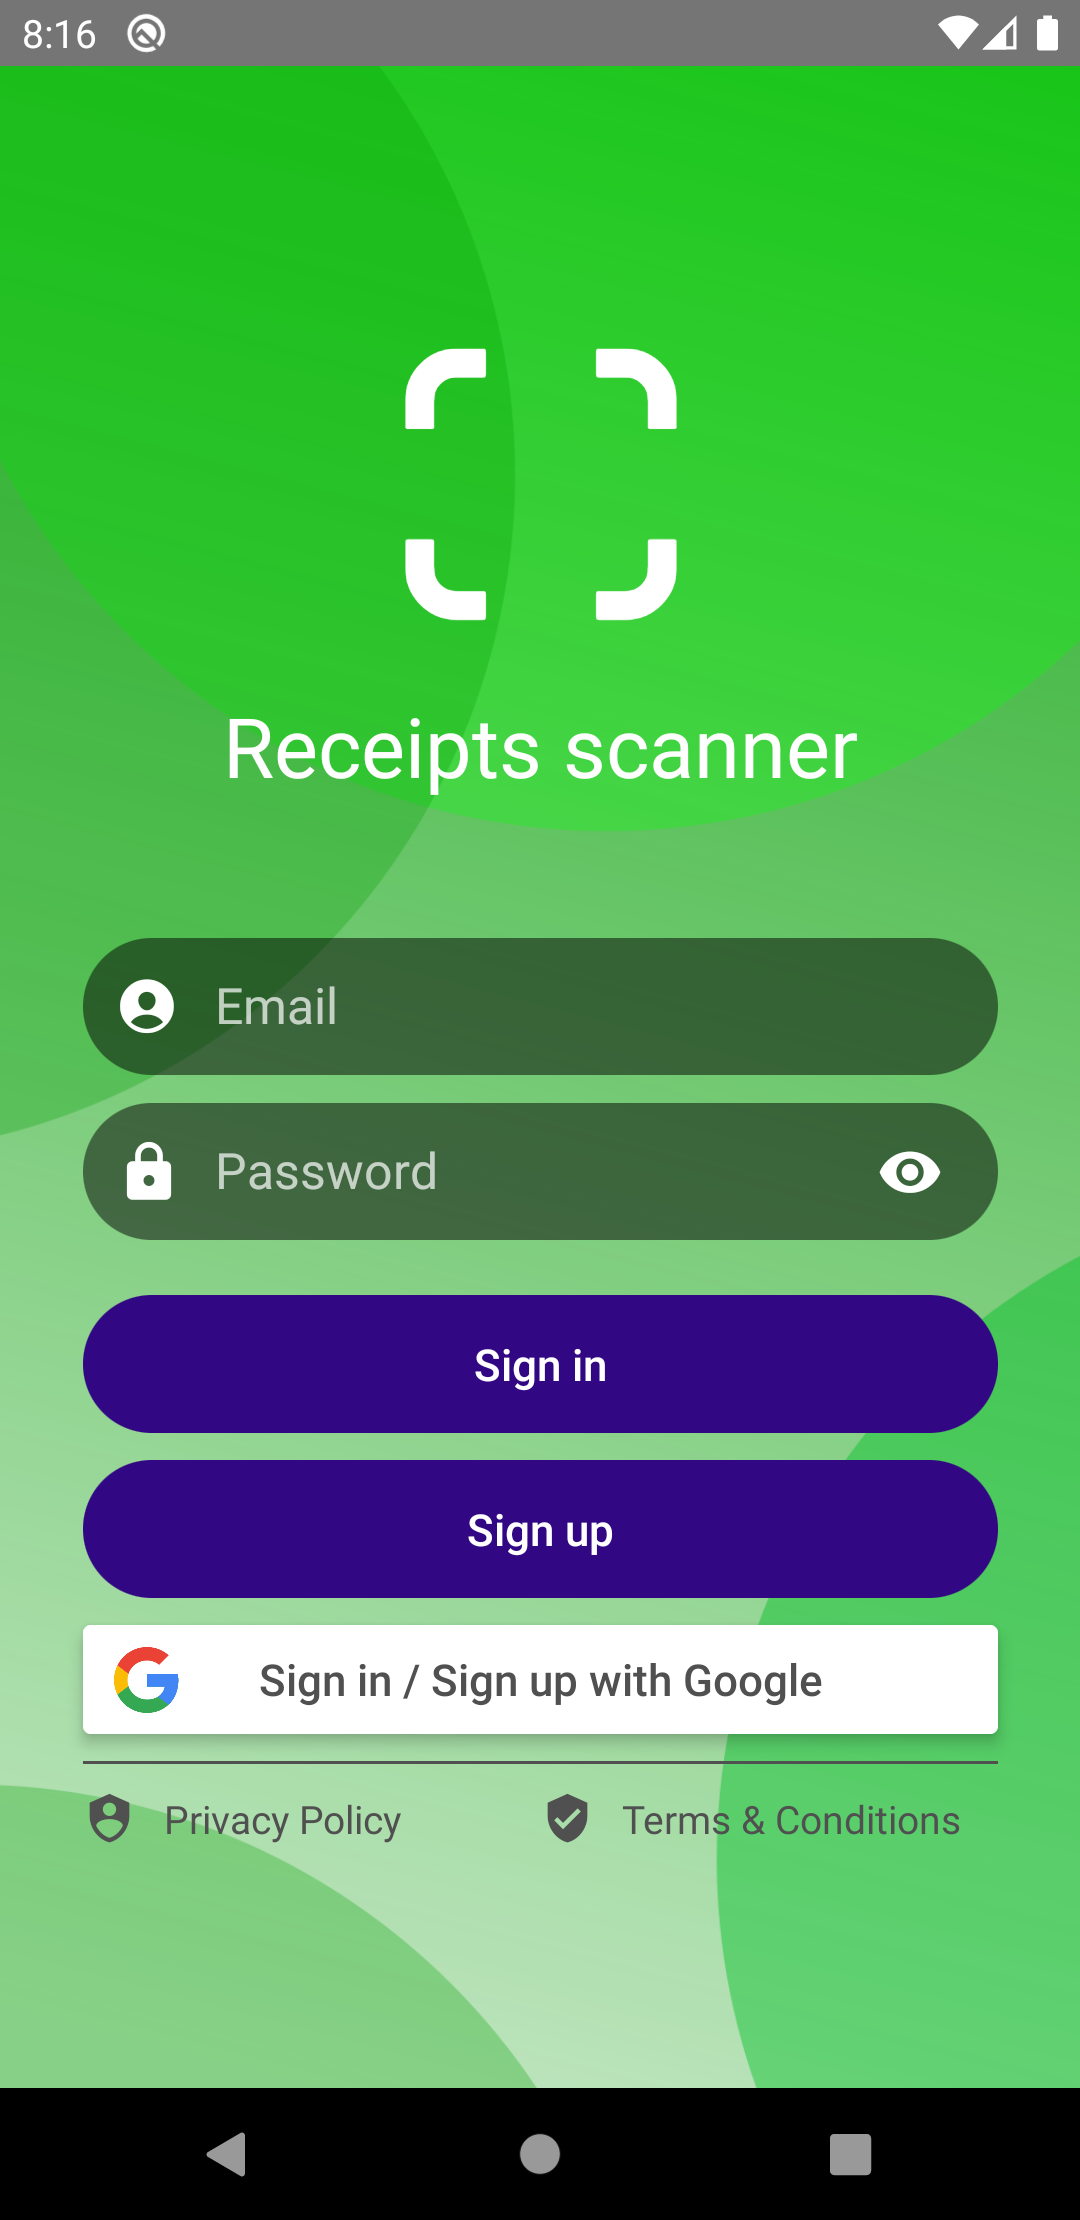
\includegraphics[width=\subfigsize\textwidth]{figures/screens/android/light/login_screen}
  \caption{Empty login form.}
  \label{fig:login_screen}
\end{subfigure}
\begin{subfigure}[t]{\half\textwidth}
  \centering
  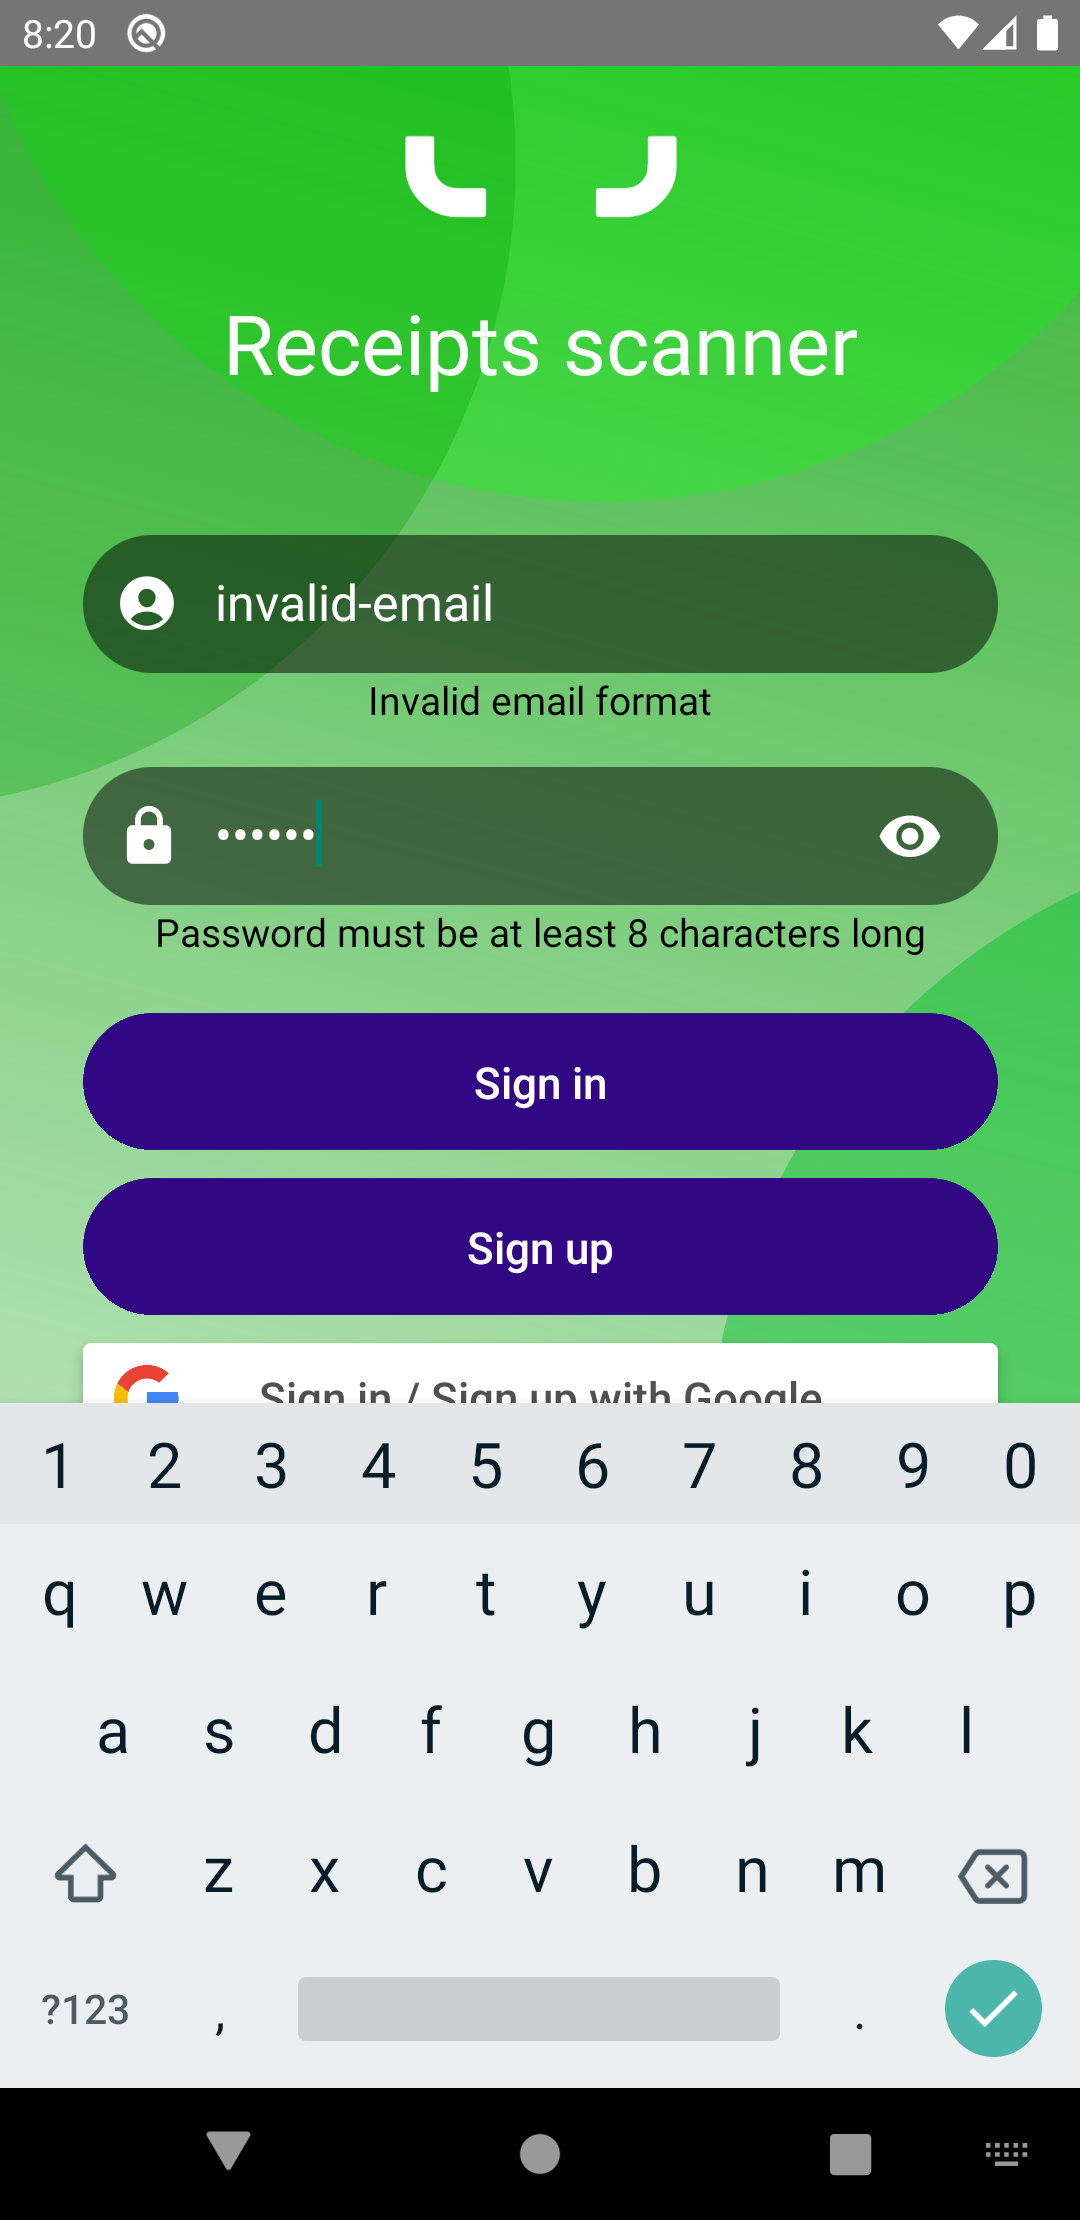
\includegraphics[width=\subfigsize\textwidth]{figures/screens/android/light/login_validation}
  % mbox -> do not hyphenate
  \caption{Form with validation \mbox{errors}.}
  \label{fig:login_validation}
\end{subfigure}
\caption{Login screen.}
\end{figure}

When the user first launches the application, a login screen is displayed. The login screen is depicted in Figure \ref{fig:login_screen}. It consists of two text input fields and three buttons. The first input field is for email, and the second is for password. It is possible to display the entered password in plain text form by pressing the eye icon next to the password input. Based on the user's preference, they can choose one of the two supported authentication mechanisms:

\begin{enumerate}
    \item \textbf{Authentication with email and password}
    
    Figure \ref{fig:sign_in_flow} shows how the process of a sign-in with email and password looks. The form offers a real-time validation, so the user is instantly notified if they have entered an invalid email or a password. The validation is shown in Figure \ref{fig:login_validation}.
    
    \begin{figure}
        \begin{center}
            \includegraphics[width=\textwidth]{figures/diagrams/Sign_in_flow}
        \end{center}
        \caption{Activity diagram of a user signing in.}
        \label{fig:sign_in_flow}
    \end{figure}
    
    Figure \ref{fig:sign_up_flow} shows the process of a sign-up with email and password.
    
    \begin{figure}
        \begin{center}
            \includegraphics[width=\textwidth]{figures/diagrams/Sign_up_flow}
        \end{center}
        \caption{Activity diagram of a user signing up.}
        \label{fig:sign_up_flow}
    \end{figure}
    
    \item \textbf{Authentication with a Google account}
    
    \phantomsection
    \label{phantom:google_sign_in}
    Figure \ref{fig:google_auth_flow} shows authentication flow using Google Sign In\footnote{Google Sign In on GitHub: \url{https://github.com/react-native-google-signin/google-signin}.} native module.
    Authentication with Google is not available in the Windows version of Receipts Scanner because the Google Sign In library does not support React Native Windows yet\footnote{GitHub issue that tracks adding of support of Google Sign In for Windows: \url{https://github.com/microsoft/react-native-windows/issues/6531}}.
    
    \begin{figure}
        \begin{center}
            \includegraphics[width=0.9\textwidth]{figures/diagrams/Google_auth_flow}
        \end{center}
        \caption{Activity diagram of a user authenticating with a Google account.}
        \label{fig:google_auth_flow}
    \end{figure}
\end{enumerate}

What all three workflows have in common is that the user's session is persisted even if the application is restarted.
If a user wanted to use a different account, they could sign out in the settings screen, depicted in Figure \ref{fig:settings_screen}. Clicking the \textit{Sign out} button ends the session and redirects the user back to the login screen.

\begin{figure}
    \begin{center}
        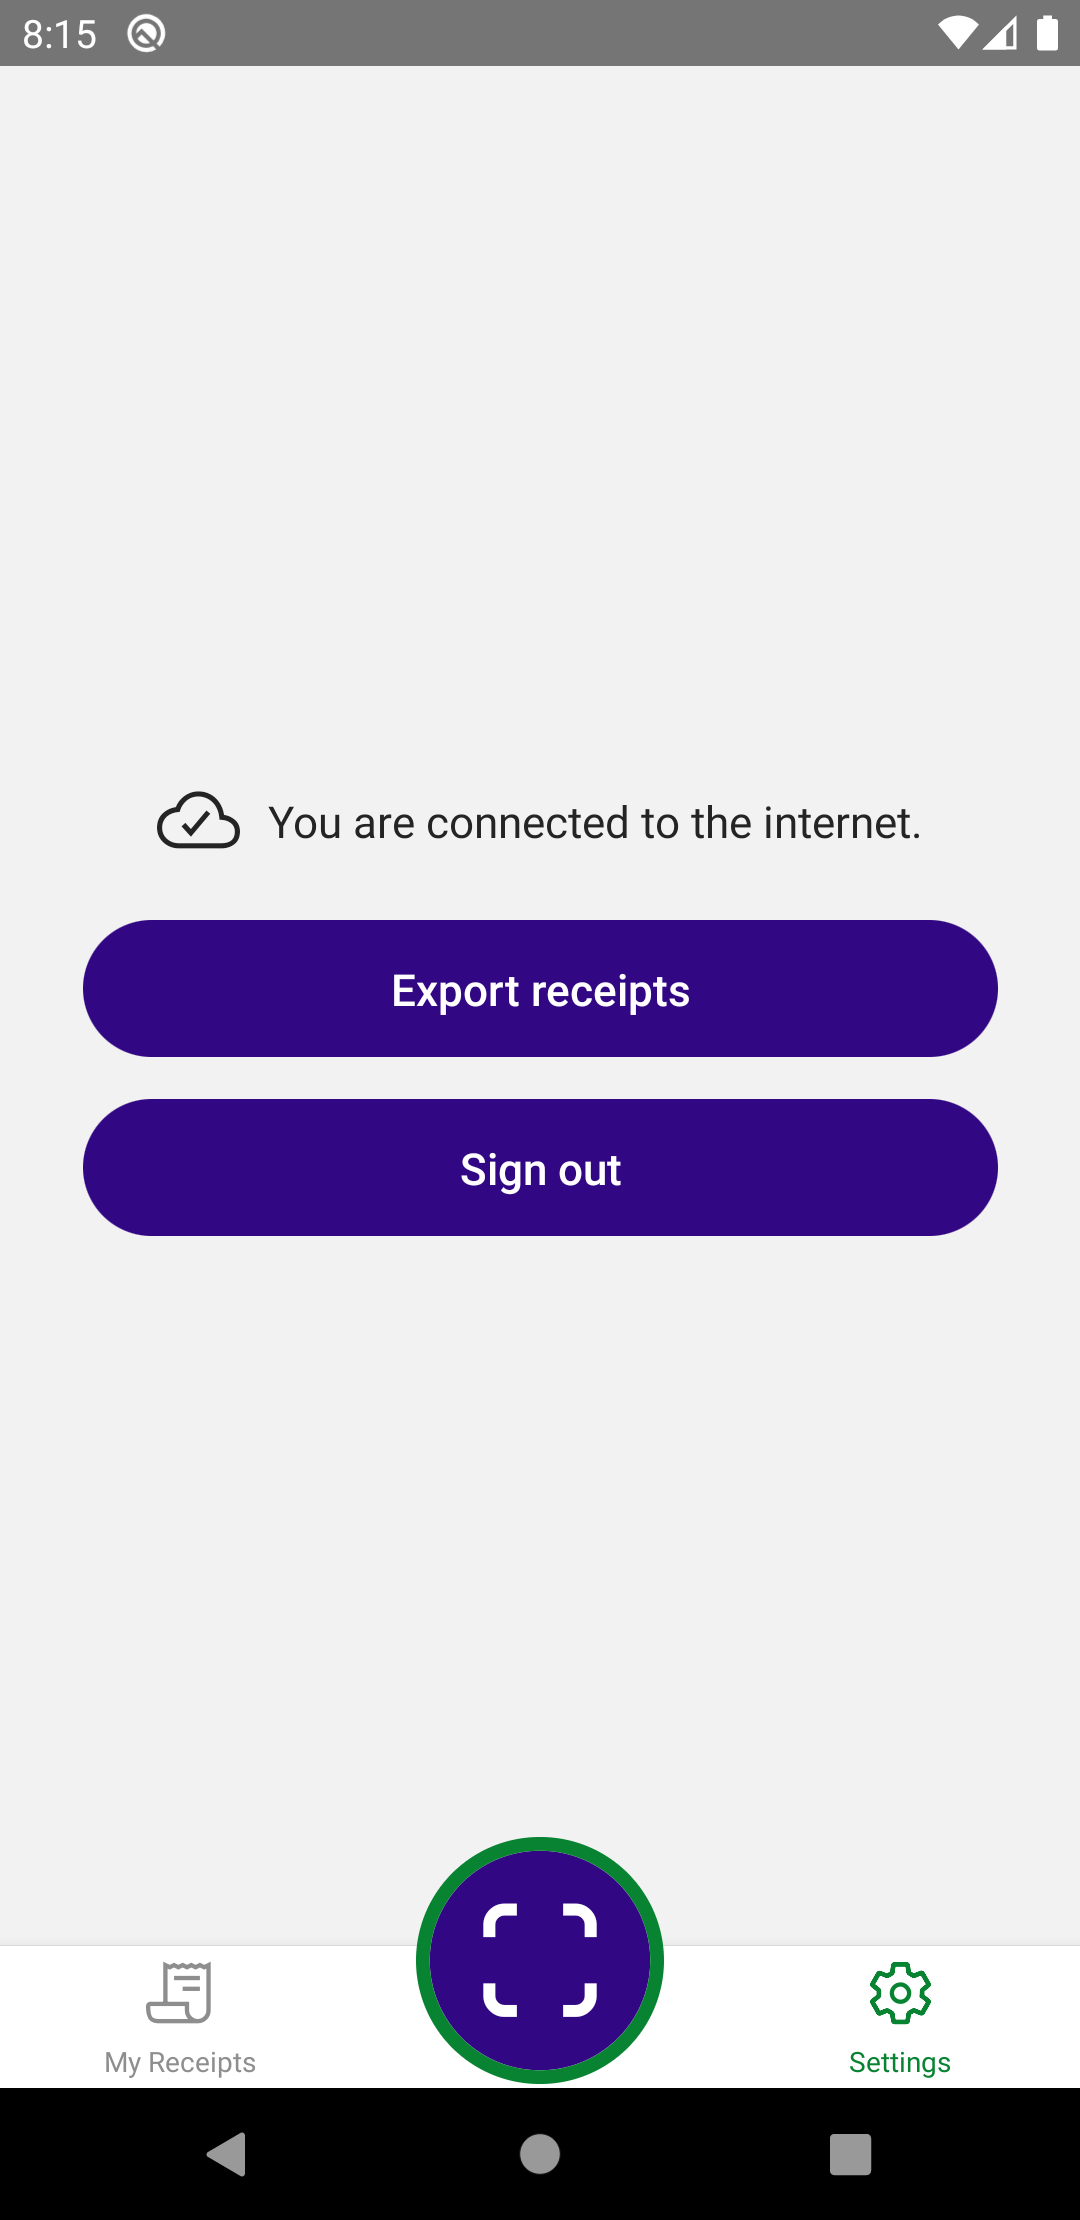
\includegraphics[width=\half\textwidth]{figures/screens/android/light/settings_screen}
    \end{center}
    \caption{Settings screen with \textit{Sign out} button.}
    \label{fig:settings_screen}
\end{figure}

\section{Adding a receipt}
The main functionality offered by Receipts Scanner is adding a receipt and storing it in the user's collection of receipts.
This process is visualized in Figure \ref{fig:add_receipt_android}.
It starts by the user selecting an already existing photo of a receipt from a gallery or by taking a new photo with the phone camera. The photo can be cropped to remove the background. It can also be rotated. The rotation does not have any effect on the result of OCR. It affects only how the photo will be shown to the user in their receipts collection.

Next, three sequences of processes happen asynchronously:

\begin{itemize}
    \item The image of the receipts is sent to Form Recognizer API. The returned data (structured text information extracted from the image) is sent to the Python API \texttt{/category} endpoint, where emojis are added to all items that have been recognized on the receipt.
    
    Form Recognizer and Python API are described in Sections \ref{sec:form_recognizer} and \ref{sec:python_api}, respectively.
    
    \item The image is uploaded to Firebase Storage.

    \item The image is sent to the Python API \texttt{/process-image} endpoint. The endpoint returns a processed grayscale image that is then uploaded to Firebase Storage.
\end{itemize}

At the end, the receipt document is added to the user's receipt collection in Google Firestore, and the edit form is shown. 

The benefit of the asynchronicity of those processes is that the whole process is much faster than if it happened synchronously. Adding a receipt takes under 8 seconds on average\footnote{Based on measurements of 10 different receipts.}.

\begin{figure}
    \begin{center}
        \includegraphics[width=\textwidth]{figures/diagrams/Add_receipt_Android}
    \end{center}
    \caption{Activity diagram of a user adding a new receipt.}
    \label{fig:add_receipt_android}
\end{figure}

\subsection{Uploading image from Windows}
On Android, the image capture and selection from the gallery is provided by library react-native-image-crop-picker\footnote{\url{https://github.com/ivpusic/react-native-image-crop-picker}}. However, this library does not support Windows. A library react-native-document-picker\footnote{\url{https://github.com/rnmods/react-native-document-picker}} used to provide a file selection feature for Windows but is incompatible with the current version of React Native for Windows. 

For this reason, a native C++ module \texttt{FilePicker} was implemented. It allows to pick an image from the Windows Explorer and returns an object containing the path to the image, MIME type\footnote{MIME (Multipurpose Internet Mail Extensions) type identifies the format of data transmitted on the internet.} and the image data encoded as Base64\footnote{\definition{Base64} is an encoding that encodes binary data into ASCII text.}. This module is then used in the JavaScript code. However, the image upload functionality is not complete on Windows because Firebase Storage for Web uses Web APIs that are not available in React Native running on Windows. An option to overcome this issue would be finding cloud storage that supports the upload of Base64 strings, preferably without any library, using only REST API.

The \texttt{FilePicker} module could be eventually released as a separate package, so that it could be used by other React Native developers.

\section{Form Recognizer}
\label{sec:form_recognizer}
\definition{Form} Recognizer is a cloud service by Microsoft for extracting structured information from documents \cite{WhatIsFormRecognizer}. It provides a pre-built model that is suitable for recognizing English receipts \cite{FormRecognizerPrebuiltReceiptModel}. It can be accessed through a JavaScript client library\footnote{\url{https://docs.microsoft.com/en-us/javascript/api/overview/azure/ai-form-recognizer-readme?view=azure-node-latest\#recognize-receipts}}. However, this library is built for Node.js runtime, which is different from the React Native runtime. In most cases, React Native uses JavaScriptCore, which is the JavaScript engine that powers Safari \cite{JavaScriptRNEnvironment}.

Receipts Scanner implements a service \texttt{FormRecognizerClient} with the same interface as the one from the official library, but it relies solely on API calls to the Form Recognizer API. The method to extract the information from the receipt is modelled as a long-running operation, which means that the initial request returns a URL to which the subsequent requests for the result should be made.

After \texttt{FormRecognizerClient} is created, its \texttt{beginRecognizeContent} method is called with the image that should be processed with the OCR service. The method returns an instance of a \texttt{Poller}. The \texttt{Poller} provides a method \texttt{pollUntilDone} that repeatedly sends requests to the Form Recognizer API until the result is available.

\section{Python API}
\label{sec:python_api}
The Python API is a service that runs separately from Receipts Scanner. It serves two purposes: to process an image of a receipt and to categorize receipt items.

It provides three endpoints\footnote{Detailed documentation of the endpoints is available at \url{https://documenter.getpostman.com/view/9355808/TzJsfdUK}.}:

\begin{itemize}
    \item \texttt{GET /} \Dash Returns a health check string. It is used to make sure that the service is running.
    
    \item \texttt{POST /category} \Dash Expects a JSON containing an item name, possibly consisting of multiple words. It returns a category of that item and an associated emoji.
    
    \item \texttt{POST /process-image} \Dash Expects a form-data containing an image. It returns a JSON containing the processed version of the image as a Base64 string and the image MIME type.
\end{itemize}

\subsection{Item categorization}
In order to make the application more visually attractive and to improve the user experience, each item on the receipt is assigned an emoji. The emoji is chosen based on the words that appear in the item name. If the user is not content with the automatically assigned emoji, they can remove it in the receipt edit form.

When a user adds a new receipt, the items on the receipt are sent to the Python API \texttt{/category} endpoint. The service contains a dictionary of category names as keys and emojis as values. Each item name is compared to all dictionary keys by using method \texttt{most\_similar\_to\_given} and the key that is most similar to the item name is returned, together with the emoji.

The method \texttt{most\_similar\_to\_given} is provided by the Magnitude library\cite{PatelEtal2018Magnitude}. Magnitude is a tool for utilizing and processing word embeddings. Word embeddings are typically real-valued vectors that encode the meaning of a word, such that the vectors that are close in the vector space are similar in their meaning \cite{Jurafsky2020Speech}. Magnitude is a fast and memory-efficient alternative to tools like Gensim\footnote{\url{https://radimrehurek.com/gensim/}}.

It uses its own vector storage file format \texttt{.magnitude}.
Popular embedding models such as Google's word2vec, Stanford's GloVe and Facebook's fastText have been pre-converted to the \texttt{.magnitude} format for download and usage\footnote{Pre-converted Magnitude models for download: \url{https://github.com/plasticityai/magnitude\#pre-converted-magnitude-formats-of-popular-embeddings-models}.}. Furthermore, each word embeddings model is available in three variants: light, medium and heavy. The difference is that medium and heavy models have advanced support for out-of-vocabulary keys\footnote{Words that do not appear in the model's vocabulary.}. The heavy model also features faster approximate K-Nearest Neighbors\footnote{A supervised machine learning algorithm for classification and regression problems.}.

Magnitude implements functions for looking up
vector representations for misspeled or out-of-vocabulary words. This means that it can handle abbreviations, which often appear on receipts, and whole sentences reasonably well.

The interface of the library is agnostic to the underlying model.
In Receipt Scanner, the fastText model is used \Dash more specifically, its medium variant, as only the exact similarity search is performed, so there is no need for faster approximate K-Nearest Neighbors. The light variant is not used because it handles item names that contain multiple words poorly.

Another constraint for choosing the model was its size. Google Cloud Run, a cloud service where the model is running, does not allow containers larger than 8 GB. Google's medium word2vec model is 4.9 GB large compared to fastText, which is only 1.6 GB large. The container with word2vec did not fit into the 8 GB limit.

The used fastText model was pre-trained on over 16 billion words from Wikipedia 2017, Statmt.org news and UMBC news \cite{Mikolov2018Advances}. It contains only English word vectors. However, fastText provides models for other languages\footnote{Word vectors for 157 languages:\\ \url{https://fasttext.cc/docs/en/crawl-vectors.html}.}, which could be converted using the Magnitude converter\footnote{\url{https://github.com/plasticityai/magnitude\#file-format-and-converter}} and used in a localized Receipts Scanner, e.g. with support for the Czech language.

Table \ref{table:models_comparison} shows results from various word embeddings models. The first two columns are produced by Google's word2vec, which was trained on 100 billion words from Google News \cite{Google2013Word2Vec}. The third column is fastText. The fourth column is fastText with subwords information. In the subwords model, each word is represented as a bag of character \textit{n}-grams. Taking the
word \textit{where} and $n = 3$ as an example, it will be
represented by the following character \textit{n}-grams:
\[
<\text{wh, whe, her, ere, re}>
\]
and the special sequence $<\text{where}>$. The less-than sign $<$ and the greater-than sign $>$ are special boundary symbols. \cite{BojanowskiEtal2017Enriching}

The results show that the case matters, e.i. \textit{CHUPA LOLLIPOPS} and \textit{Chupa lollipops} are categorized differently, and how more concrete terms are mapped to more general terms, e.i. \textit{salmon} and \textit{cola} are categorized as \textit{fish} and \textit{cold beverage} respectively.

\begin{table}
    \begin{tabular}{>{\bfseries}L{0.2\textwidth}L{0.2\textwidth}L{0.2\textwidth}L{0.2\textwidth}L{0.2\textwidth}}
        \toprule
        \textbf{item name} & \textbf{word2vec light} & \textbf{word2vec medium} & \textbf{fastText medium} & \textbf{fastText subwords medium}\\
        \midrule
salty snack & \emoji{santa-claus} santa claus & \emoji{pretzel} snack & \emoji{pretzel} snack & \emoji{pretzel} snack\\
CHUPA \mbox{LOLLIPOPS} & \emoji{field-hockey} field hockey & \emoji{candy} candy & \emoji{candy} candy & \emoji{lollipop} lollipop\\
Chupa \mbox{lollipops} & \emoji{floppy-disk} floppy disk & \emoji{candy} candy & \emoji{lollipop} lollipop & \emoji{lollipop} lollipop\\
salmon & \emoji{fish} fish & \emoji{fish} fish & \emoji{fish} fish & \emoji{fish} fish\\
shampoo & \emoji{lotion-bottle} lotion & \emoji{lotion-bottle} lotion & \emoji{lotion-bottle} lotion & \emoji{lotion-bottle} lotion\\
ipad air & \emoji{dashing-away} air condition & \emoji{mobile-phone} iphone & \emoji{mobile-phone} iphone & \emoji{mobile-phone} iphone\\
manual weight & \emoji{womans-hat} woman’s hat & \emoji{weight-lifting}️ weight lifting & \emoji{weight-lifting}️ weight lifting & \emoji{weight-lifting} weight lifting\\
frozen pizza & \emoji{hot-pepper}️ hot pepper & \emoji{pizza} pizza & \emoji{pizza} pizza & \emoji{pizza} pizza\\
Cola 1 l & \emoji{womans-sandal} woman’s sandal & \emoji{potable-water} cold beverage & \emoji{potable-water} cold beverage & \emoji{chocolate-bar} chocolate bar\\
eggs & \emoji{egg} egg & \emoji{egg} egg & \emoji{egg} egg & \emoji{egg} egg\\
T MAT \mbox{CHEDDAR} & \emoji{floppy-disk} floppy disk & \emoji{cheese-wedge} cheese & \emoji{cheese-wedge} cheese & \emoji{cheese-wedge} cheese\\
pork loin chop & \emoji{motor-scooter} motor scooter & \emoji{hot-dog} hot dog & \emoji{pig} pork & \emoji{pig} pork\\
        \bottomrule
    \end{tabular}
    \caption{Comparison of pretrained word embeddings models.}
    \label{table:models_comparison}
\end{table}

\subsection{Image processing}
The image processing happens independently of the OCR. The image sent to the Form Recognizer API is the original image because it uses its own image processing techniques and provides better results on original images.

The purpose of image processing in the Receipts Scanner is to provide a cleaner preview of the receipt for the user. The result is a cropped picture with black text on a white background. The whole process consists of the following steps:

\begin{enumerate}
    \item \textbf{Image loading} 
    
    The image is loaded in a grayscale.
    
    \item \textbf{Noise removal} 

    Gaussian blur is applied to reduce the Gaussian noise in the image. It is the most common type of noise in an image \cite{Shreya2019OCRCNN}. The blur is achieved by convolving the image with a Gaussian function.
    
    \begin{equation}
    G(x,y) = \frac{1}{2\pi\sigma^2}e^{-\frac{x^2+y^2}{2\sigma^2}}\text{,}
    \end{equation}
    
    where $x$ and $y$ are the distances from the origin in the horizontal and vertical axis, respectively. $\sigma$ is the standard deviation of the Gaussian distribution. \cite{Shreya2019OCRCNN}
    
    A result of applying Gaussian blur is shown in Figure \ref{fig:gaussian_blur}.
    
    \begin{figure}
        \centering
        \begin{subfigure}[t]{\half\textwidth}
          \centering
          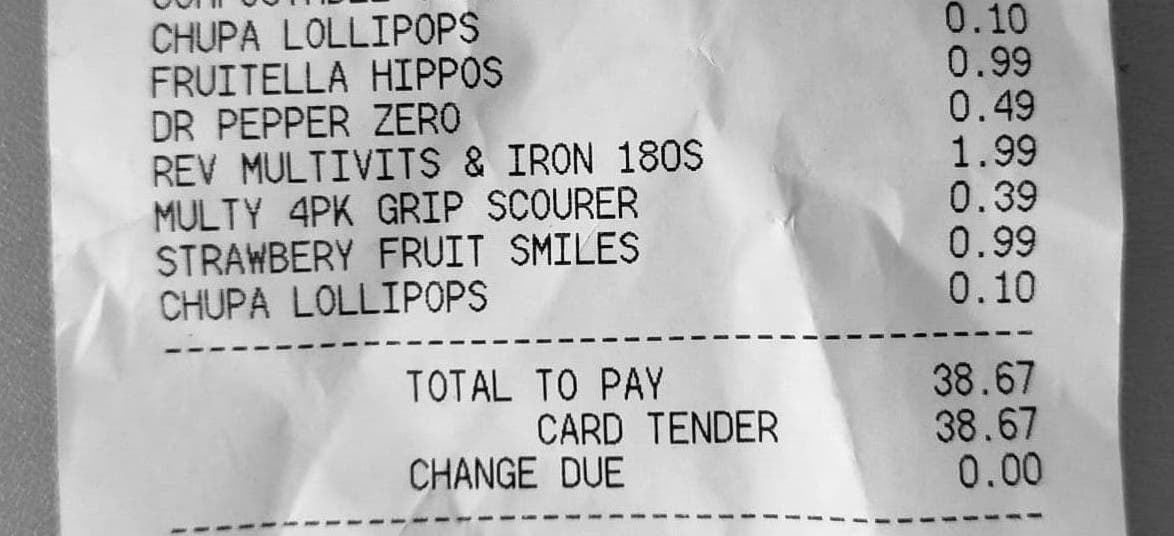
\includegraphics[width=\subfigsize\textwidth]{figures/image_processing/before_blur}
          \caption{Before Gaussian blur.}
        \end{subfigure}
        \begin{subfigure}[t]{\half\textwidth}
          \centering
          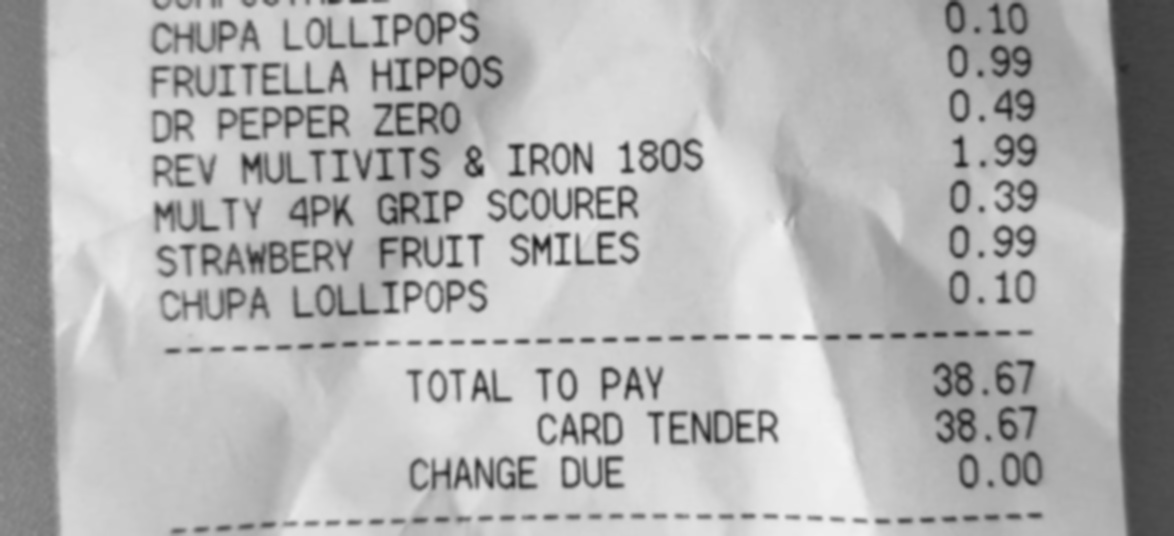
\includegraphics[width=\subfigsize\textwidth]{figures/image_processing/after_blur}
          \caption{After Gaussian blur.}
        \end{subfigure}
        \caption{Comparison of an image before and after Gaussian blur has been applied.}
        \label{fig:gaussian_blur}
    \end{figure}
    
    \item \textbf{Binary thresholding}
    
    It is beneficial to convert the images to binary images to detect the edges and contours better. Binary thresholding sets pixel value to the maximum value \Dash usually 255 (white) \Dash if its value is greater than the threshold. Otherwise, the pixel value is set to 0 (black).
    
    \begin{equation}
    \label{eqn:binary_tresholding}
    dst(x,y) = \begin{cases}
                \texttt{maxval} & \text{if }src(x,y) > \texttt{thresh}\\
                    0 & \text{otherwise}
              \end{cases}
    \end{equation}
    
    In equation \ref{eqn:binary_tresholding} $src(x,y)$ is a value of a source pixel on coordinates $x$ and $y$ and $dst(x,y)$ is a value of destination, i.e. resulting pixel, on coordinates $x$ and $y$.
    
    The threshold value can be either fixed, e.g. 127, or computed from the image. Finding the right value for the fixed thresholding is challenging, and each image might have a different optimal threshold value.
    
    Otsu's thresholding calculates the threshold value dynamically from the histogram of each image, such that the found threshold maximizes the between-class variance \cite{Gonzalez2008Digital}. Classes are black and white pixels.
    
    Figure \ref{fig:binary_threshold} shows a result of applying fixed binarization with a threshold value of 127. The edges of the receipt in this image would not be correctly recognized because the threshold value is too small.
    
    Figure \ref{fig:otsu_threshold} shows a result of applying Otsu's thresholding, which automatically found a threshold value of 151. The edges are clearly visible.
    
    \begin{figure}
        \centering
        \begin{subfigure}[t]{\half\textwidth}
          \centering
          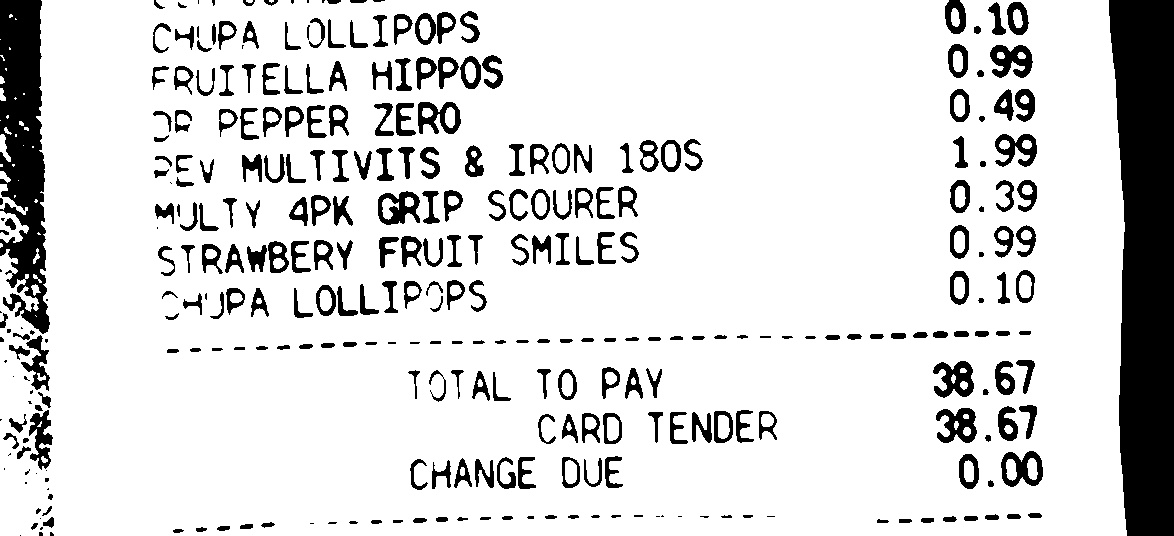
\includegraphics[width=\subfigsize\textwidth]{figures/image_processing/binary_threshold}
          \caption{Binarized image with fixed threshold of 127.}
          \label{fig:binary_threshold}
        \end{subfigure}
        \begin{subfigure}[t]{\half\textwidth}
          \centering
          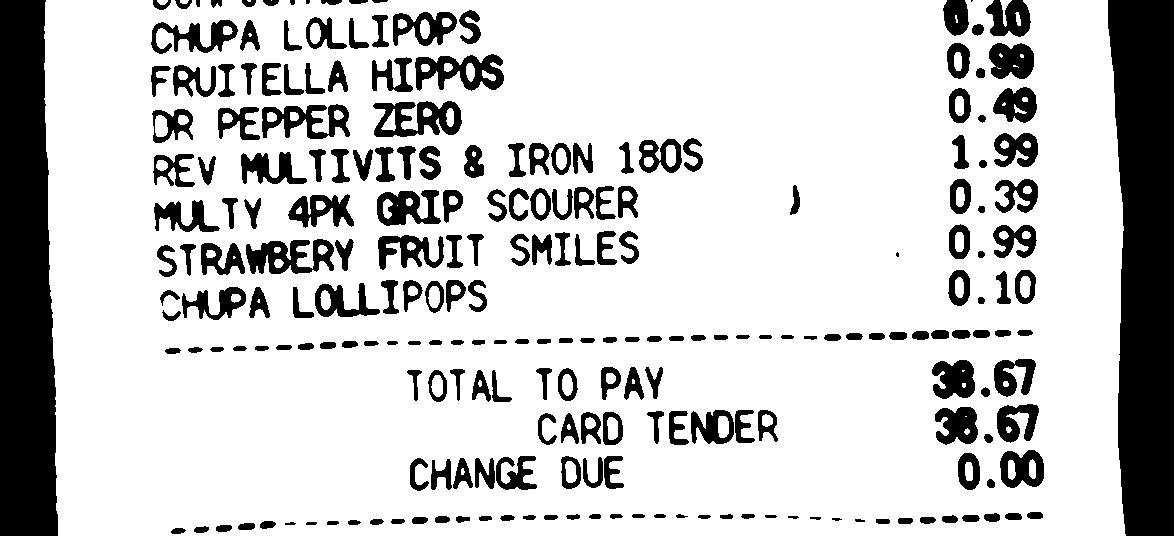
\includegraphics[width=\subfigsize\textwidth]{figures/image_processing/otsu_threshold}
          \caption{Binarized image with threshold of 151 found by Otsu's method.}
          \label{fig:otsu_threshold}
        \end{subfigure}
        \caption{Comparison of a fixed and Otsu's thresholding.}
        \label{fig:threshold_comparison}
    \end{figure}

    \item \textbf{Dilation}

    In order to determine the edges of the receipt more easily, the image is dilated. Dilation increases the size of the grid lines.
    
    Before performing dilation, the image has to be inverted. Otherwise, an opposite effect, erosion, would be achieved. It is necessary to invert the image back before contour detection, which is described in the next step.
    
    A kernel slides through the image the same way as in 2D convolution. A pixel is considered white if at least one pixel in the original image under the kernel is white.
    
    A result of applying dilation is shown in Figure \ref{fig:dilation}.
    
    \begin{figure}
        \centering
        \begin{subfigure}[t]{\half\textwidth}
          \centering
          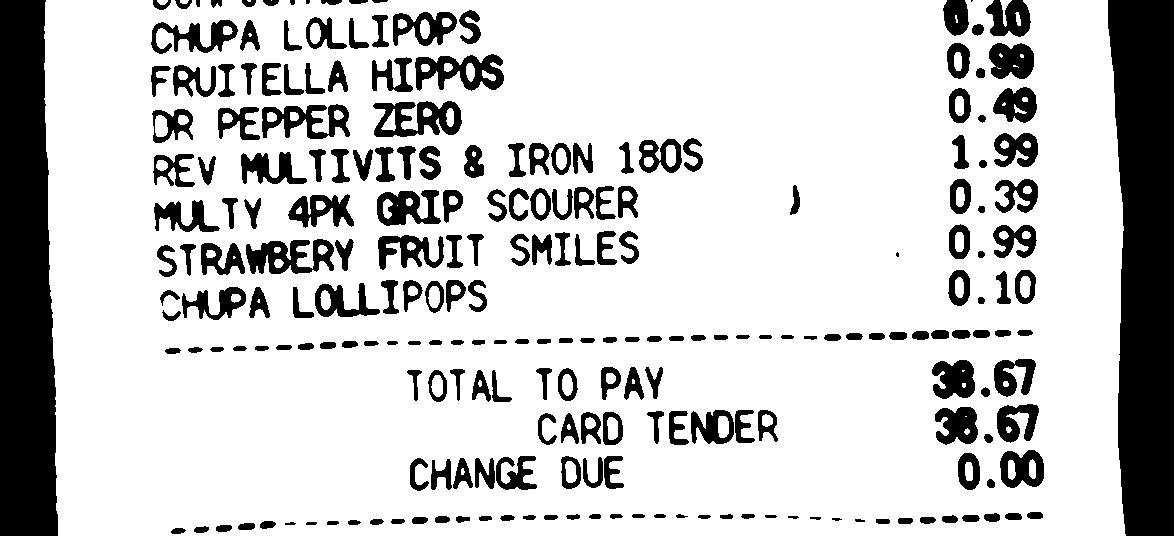
\includegraphics[width=\subfigsize\textwidth]{figures/image_processing/before_dilation}
          \caption{Before dilation.}
        \end{subfigure}
        \begin{subfigure}[t]{\half\textwidth}
          \centering
          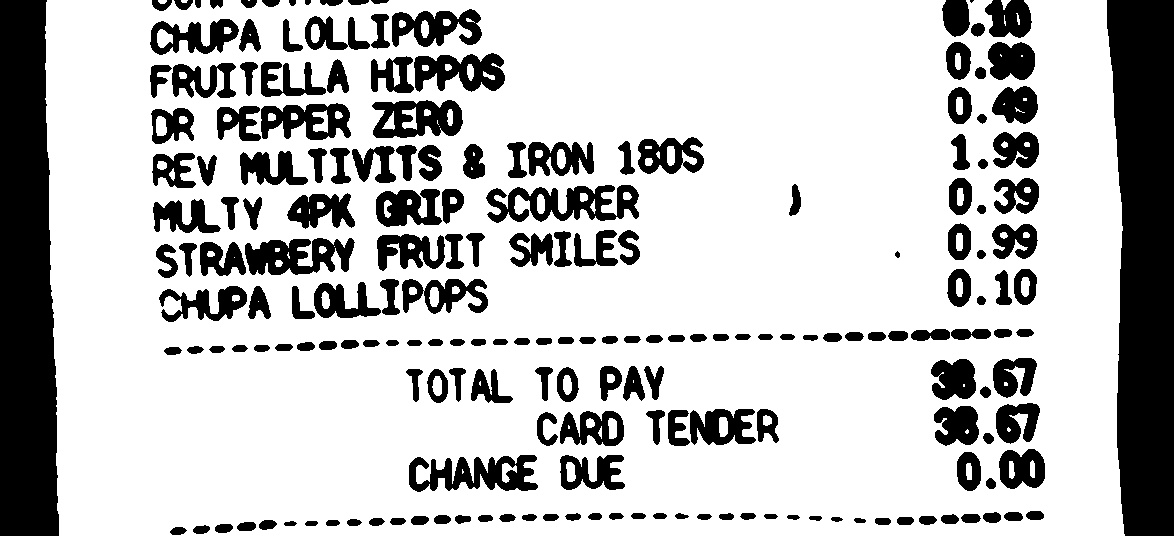
\includegraphics[width=\subfigsize\textwidth]{figures/image_processing/after_dilation}
          \caption{After dilation.}
        \end{subfigure}
        \caption{Comparison of an image before and after dilation has been applied.}
        \label{fig:dilation}
    \end{figure}

    \item \textbf{Finding the corners of a receipt}
    
    As the next step, all external contours in the image are found. Contour is a curve joining points of the same color and intensity. The contour with the largest area is most probably the contour of a receipt. Four points that represent the corners of the receipt are then found in the contour and returned. A result of this step is visualized in Figure \ref{fig:points_and_edges}.

    However, if the contour area is smaller than 30\% of the overall image, the next step, \textit{Cropping and warping}, is skipped.
    
    \begin{figure}
        \begin{center}
            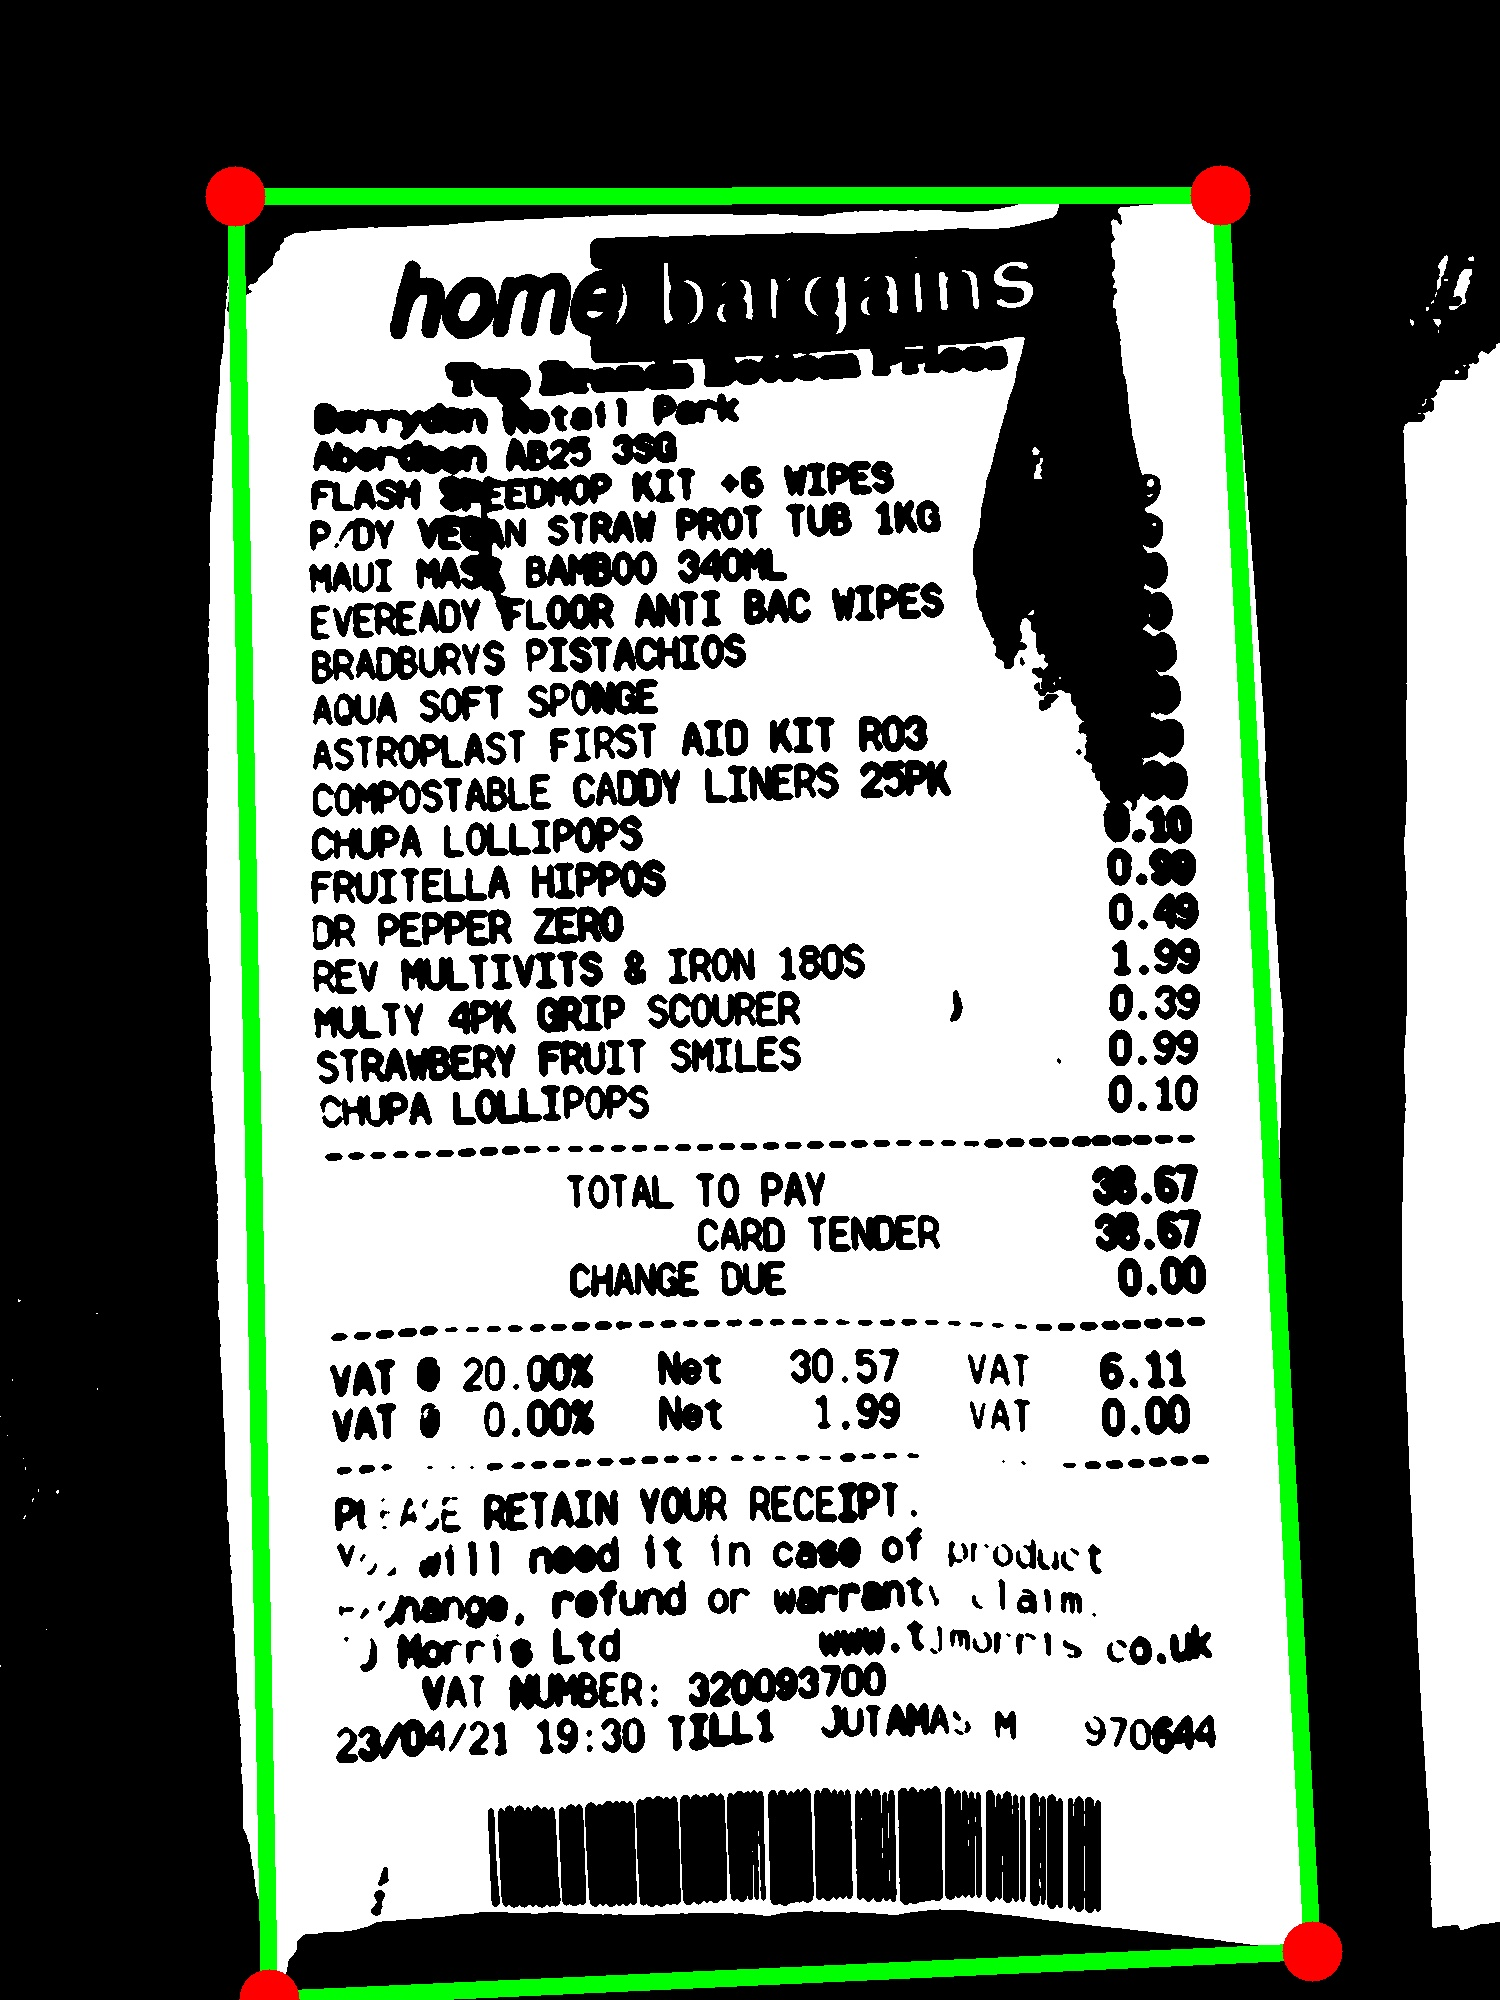
\includegraphics[width=\half\textwidth]{figures/image_processing/points_and_edges}
        \end{center}
        \caption{Binarized photo with recognized corners.}
        \label{fig:points_and_edges}
    \end{figure}

    \item \textbf{Preparing underlying picture}

    The previous steps were used to find the corners of a receipt. Although Otsu's thresholding made the edges of the white receipt clearly distinguishable from the dark background, the text of the receipt became unreadable.
    
    TODO A different scenario would be for receipt scans. Since scans usually do not have any background, Otsu's thresholding maximizes the contrast between the paper and the text instead of the contrast between the paper and the background.
    
    For receipt photos, adaptive thresholding is a better choice. This is also caused by shades in the photos, which are not present in scans.
    
    With adaptive thresholding, the threshold value for each pixel is based on a small region around it. This method gives better results for images with varying illumination. \cite{OpenCVThresholding}
    
    OpenCV library provides two methods of computing the adaptive threshold. It can be computed as the mean of the neighborhood area minus a constant $C$ or as a Gaussian-weighted sum of the neighborhood values minus the constant $C$. Empirically, the Gaussian method with $C = 2$ produced the best results.
    
    Before the adaptive thresholding is applied, the original image is blurred using Gaussian blur. This improves the result significantly, as can be seen in Figure \ref{fig:adaptive_thresholding}.
    
    \begin{figure}
        \centering
        \begin{subfigure}[t]{\half\textwidth}
          \centering
          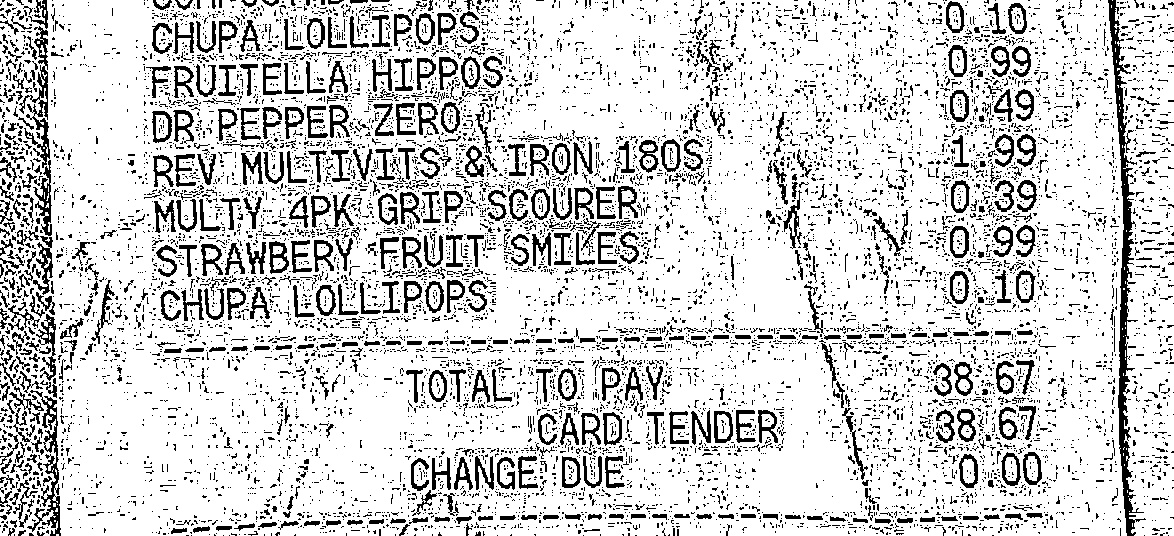
\includegraphics[width=\subfigsize\textwidth]{figures/image_processing/adaptive_thresholding_no_blur}
          \caption{Adaptive thresholding without Gaussian blur.}
        \end{subfigure}
        \begin{subfigure}[t]{\half\textwidth}
          \centering
          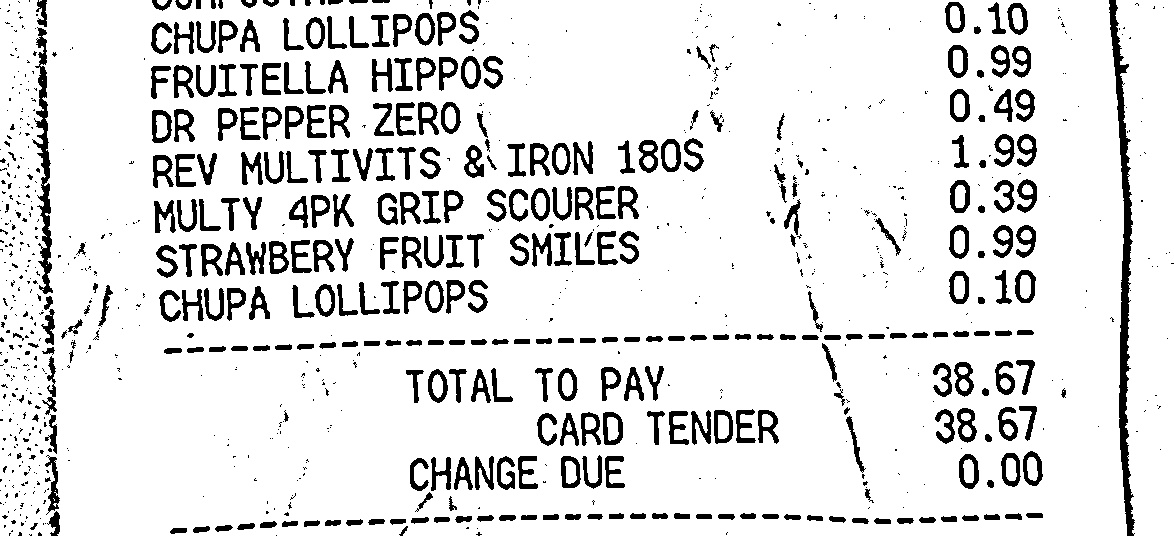
\includegraphics[width=\subfigsize\textwidth]{figures/image_processing/adaptive_thresholding}
          \caption{Adaptive thresholding after Gaussian blur.}
        \end{subfigure}
        \caption{Comparison of an adaptive thresholding with and without Gaussian blur being applied first.}
        \label{fig:adaptive_thresholding}
    \end{figure}

    \item \textbf{Cropping and warping}

    Lastly, a perspective transformation (warping) is applied to the underlying photo produced by the previous step.
    The found quadrilateral, represented by four corners, is warped into a rectangle of a similar size. This step also crops the receipt from the background. 
    
    \end{enumerate}
    
    A comparison of the original image and the final processed image is shown in Figure \ref{fig:original_vs_processed}.
    
    \begin{figure}
        \centering
        \begin{subfigure}[t]{\half\textwidth}
          \centering
          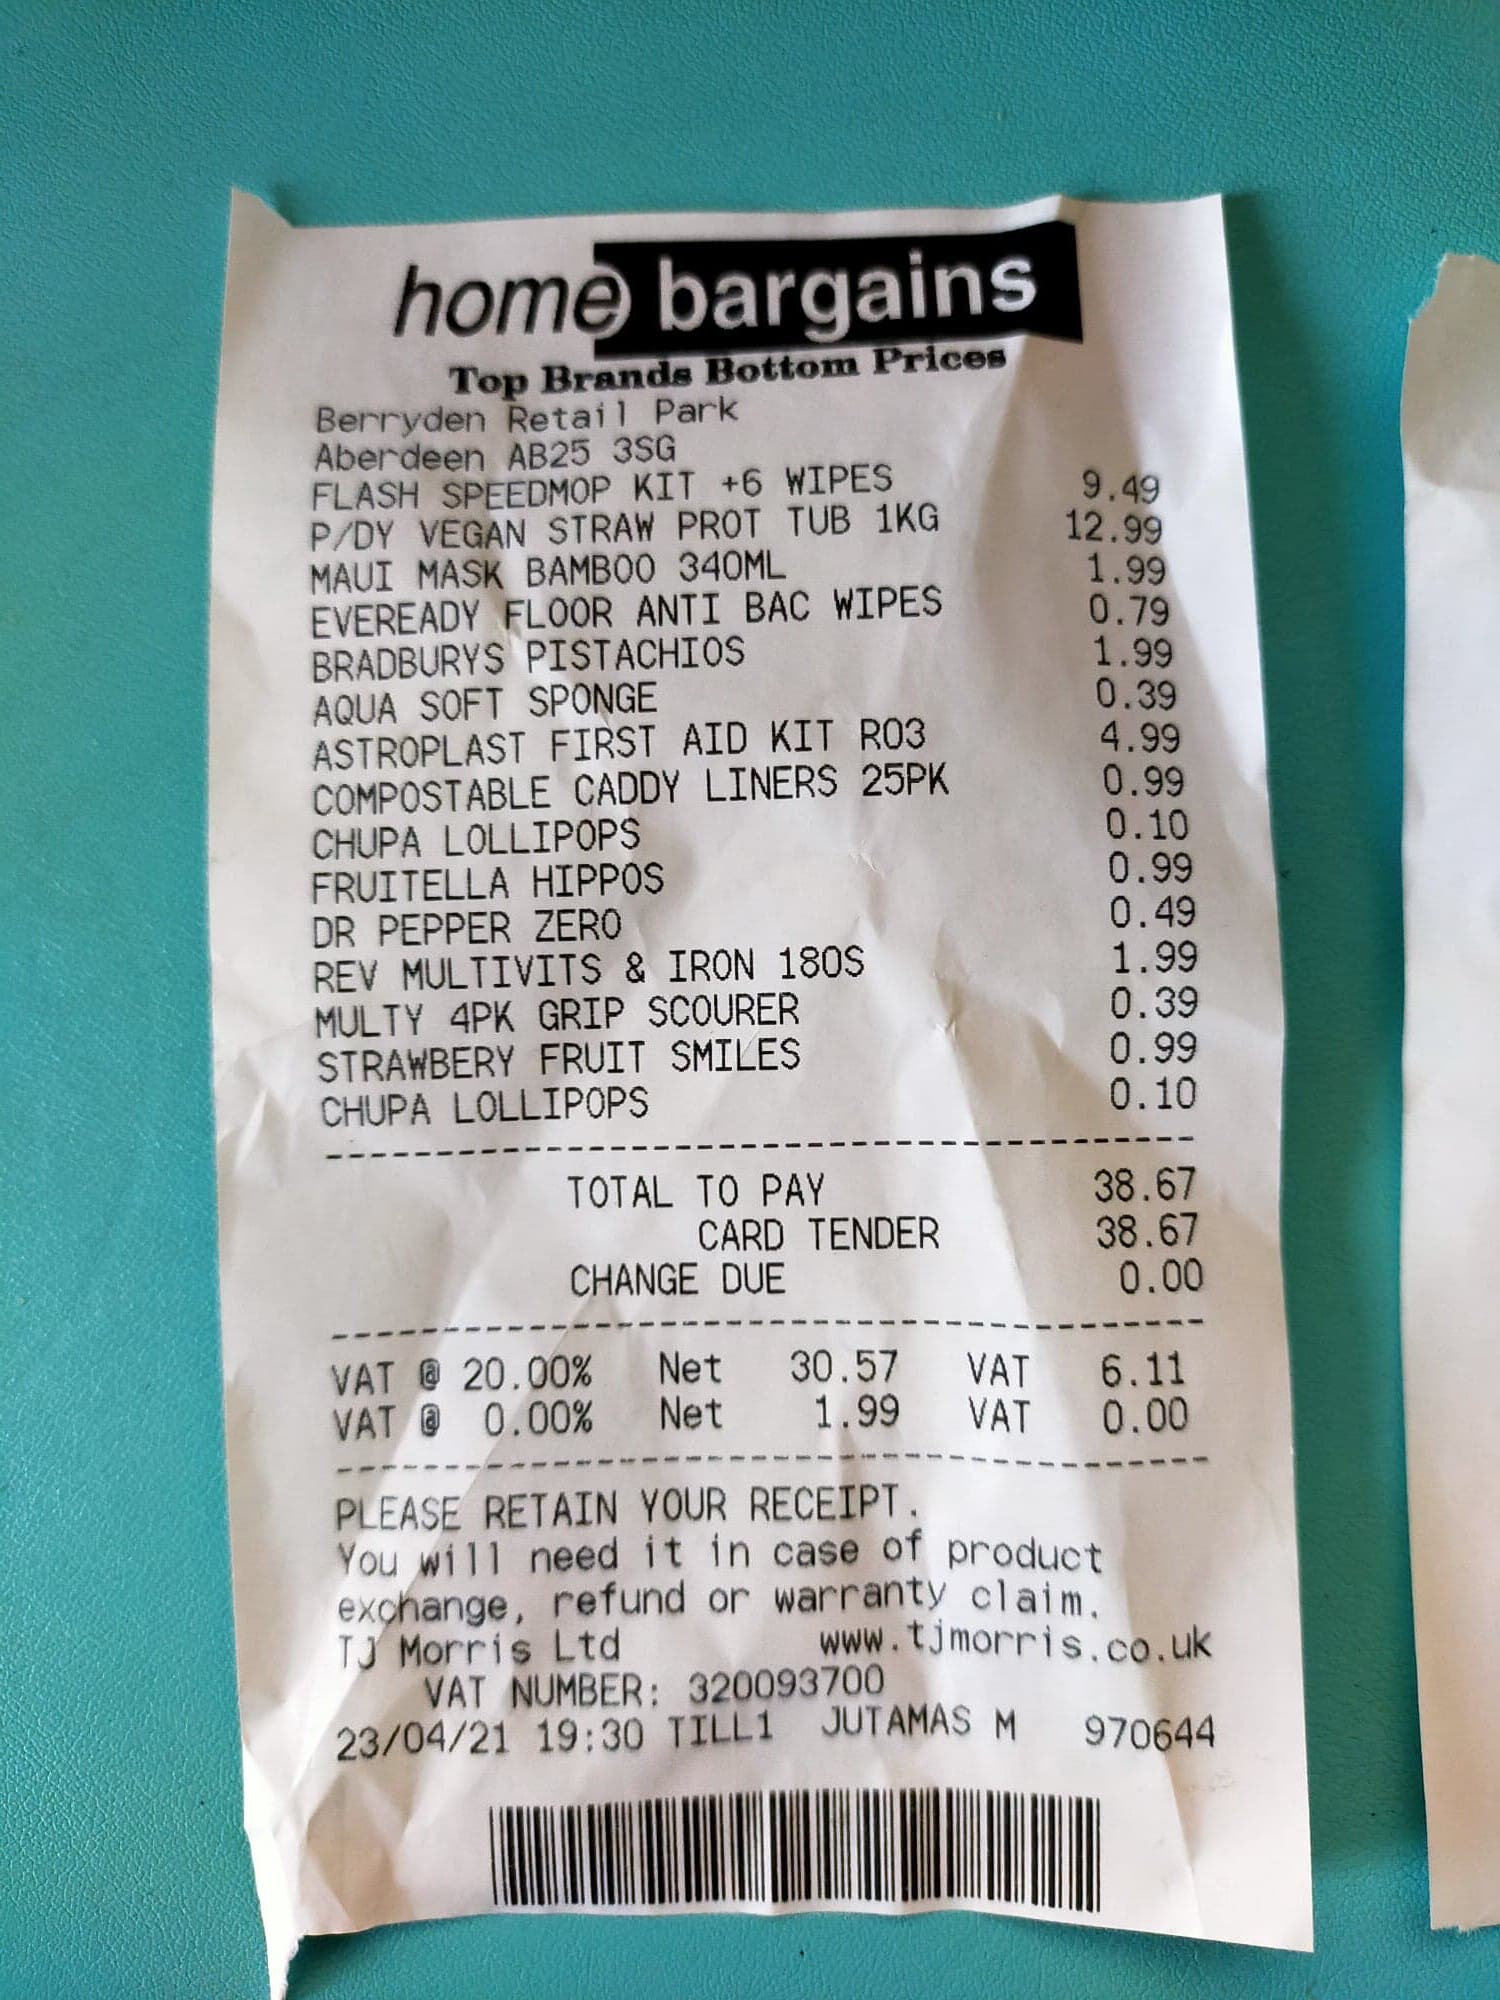
\includegraphics[width=\subfigsize\textwidth]{figures/image_processing/original_image}
          \caption{Original image.}
        \end{subfigure}
        \begin{subfigure}[t]{\half\textwidth}
          \centering
          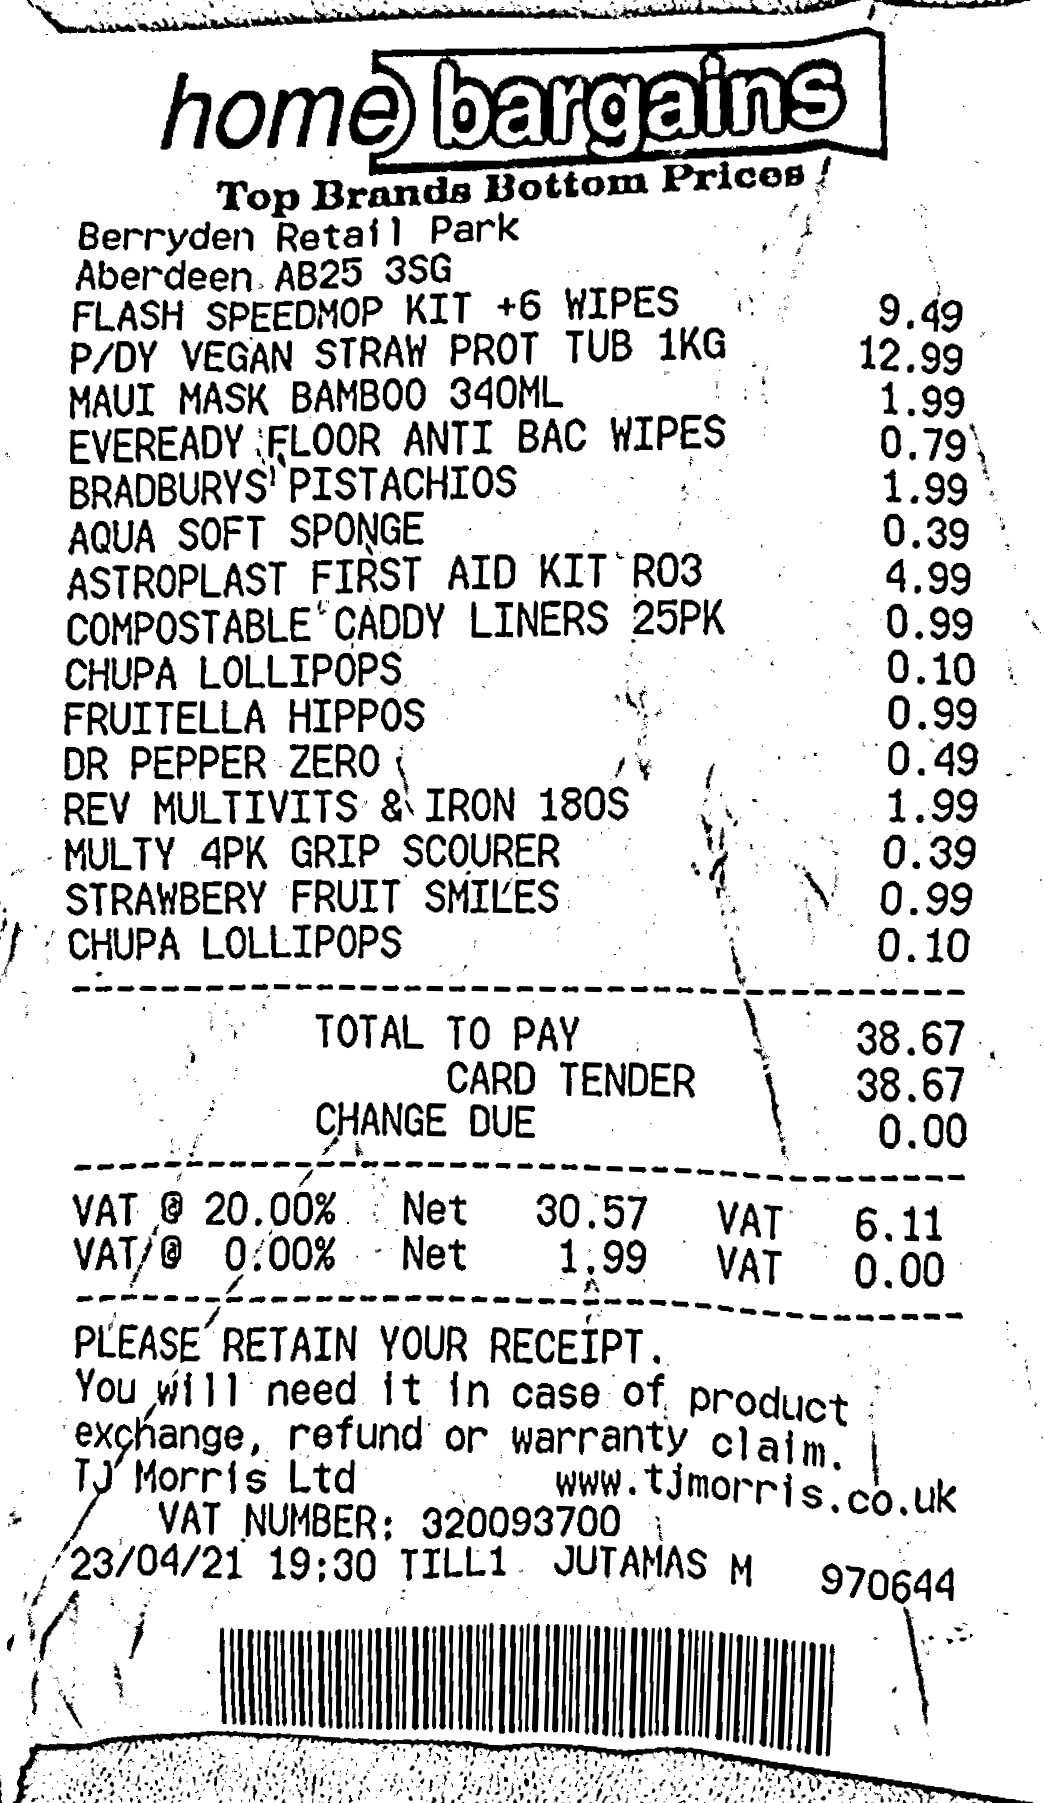
\includegraphics[width=\subfigsize\textwidth]{figures/image_processing/processed_image}
          \caption{A processed image after adaptive binarization and perspective transformation.}
        \end{subfigure}
        \caption{Comparison of a fixed and Otsu's thresholding.}
        \label{fig:original_vs_processed}
    \end{figure}

\subsection{Deployment}
The Python API is a Flask\footnote{\url{https://flask.palletsprojects.com/en/1.1.x/}} server. 
It is automatically deployed after each push to the master branch.
First, Google Cloud Build\footnote{\url{https://cloud.google.com/build}} builds a Docker image that contains the source files, external dependencies and the Magnitude word embeddings model. The built image is saved into Google Container Registry\footnote{\url{https://cloud.google.com/container-registry}}. Google Cloud Run\footnote{\url{https://cloud.google.com/run}} then runs the image in a container.
If the image is not built successfully or the Python API service fails to start, the previously deployed service stays available.

The newly deployed Python API service is tested with tests that run in the repository CI pipeline.

\section{Styles}
Apart from black and white, the Receipts Scanner user interface uses two main colors. The primary color is malachite, \texttt{\#078331} \testclr[HTML]{078331} and the secondary is \texttt{\#310783} \testclr[HTML]{310783}. The primary color has been chosen to resemble the color of banknotes. The secondary color is one of the three colors of malachite's triadic colors\footnote{The color triad was generated using color-hex tool available at \url{https://www.color-hex.com/color/078331}.}. 
The colors are chosen with respect to the contrast ratio between each other as well as the contrast ratio between those two colors and black and white. This is especially important in the dark mode.

Most of the elements are styled with these two colors to ensure a clean and consistent user interface look.

\subsection{Dark mode}
Receipts scanner switches automatically into the dark mode based on the user's device settings. The dark mode is a popular feature among users. It helps reduce digital eye strain and saves battery on devices with OLED\footnote{Unlike LCD screens that illuminate using a back panel that always lights up completely, in OLED displays, each pixel is individually lit.} screen.

Figure \ref{fig:dark_mode_android} shows the user interface with the dark mode enabled on an Android device. Figure \ref{fig:dark_mode_windows} shows the application in dark mode on Windows.

\begin{figure}
    \centering
    \begin{subfigure}[t]{\half\textwidth}
      \centering
      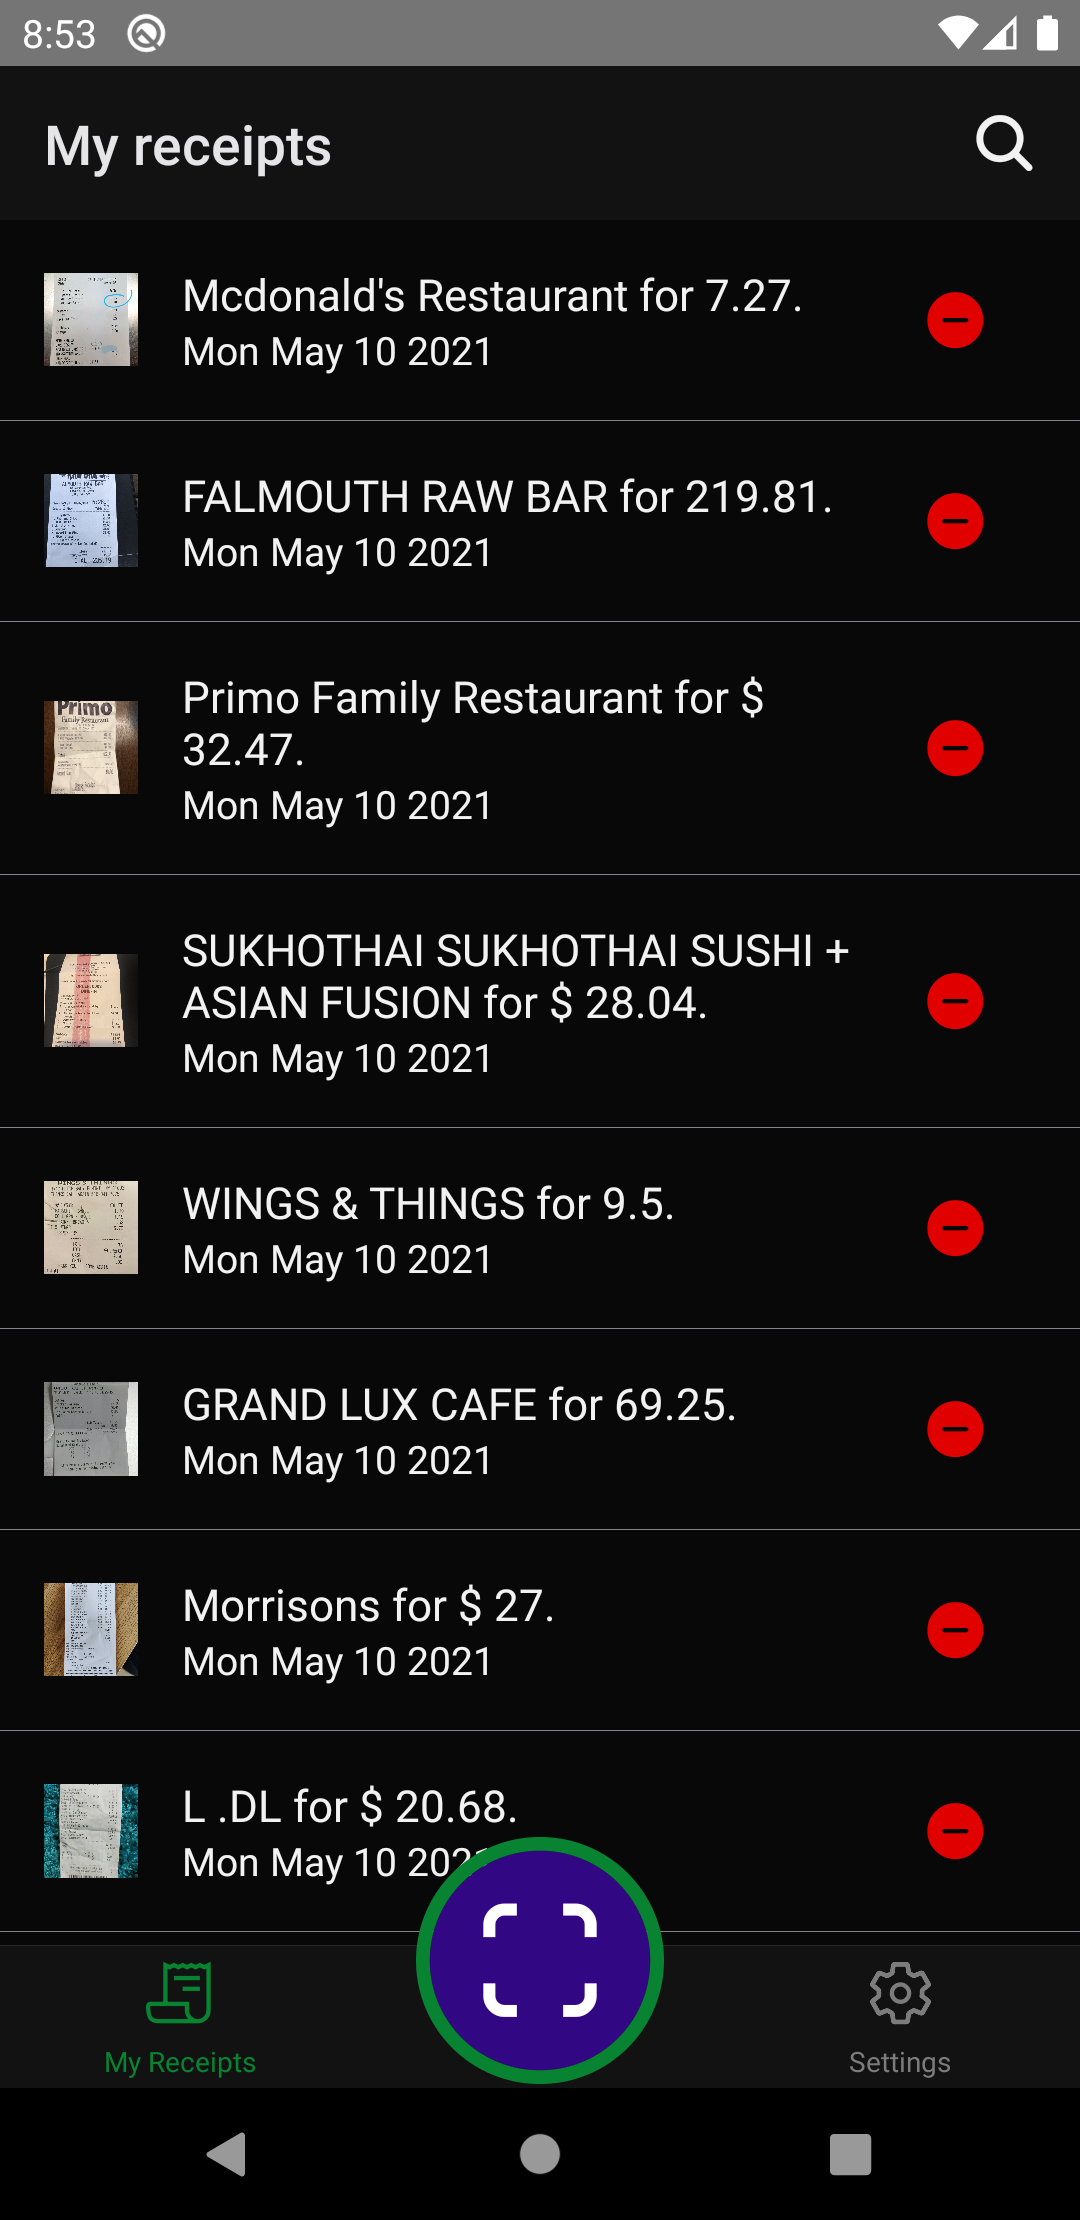
\includegraphics[width=\subfigsize\textwidth]{figures/screens/android/dark/receipts_list}
      \caption{Main application screen showing list of receipts.}
    \end{subfigure}
    \begin{subfigure}[t]{\half\textwidth}
      \centering
      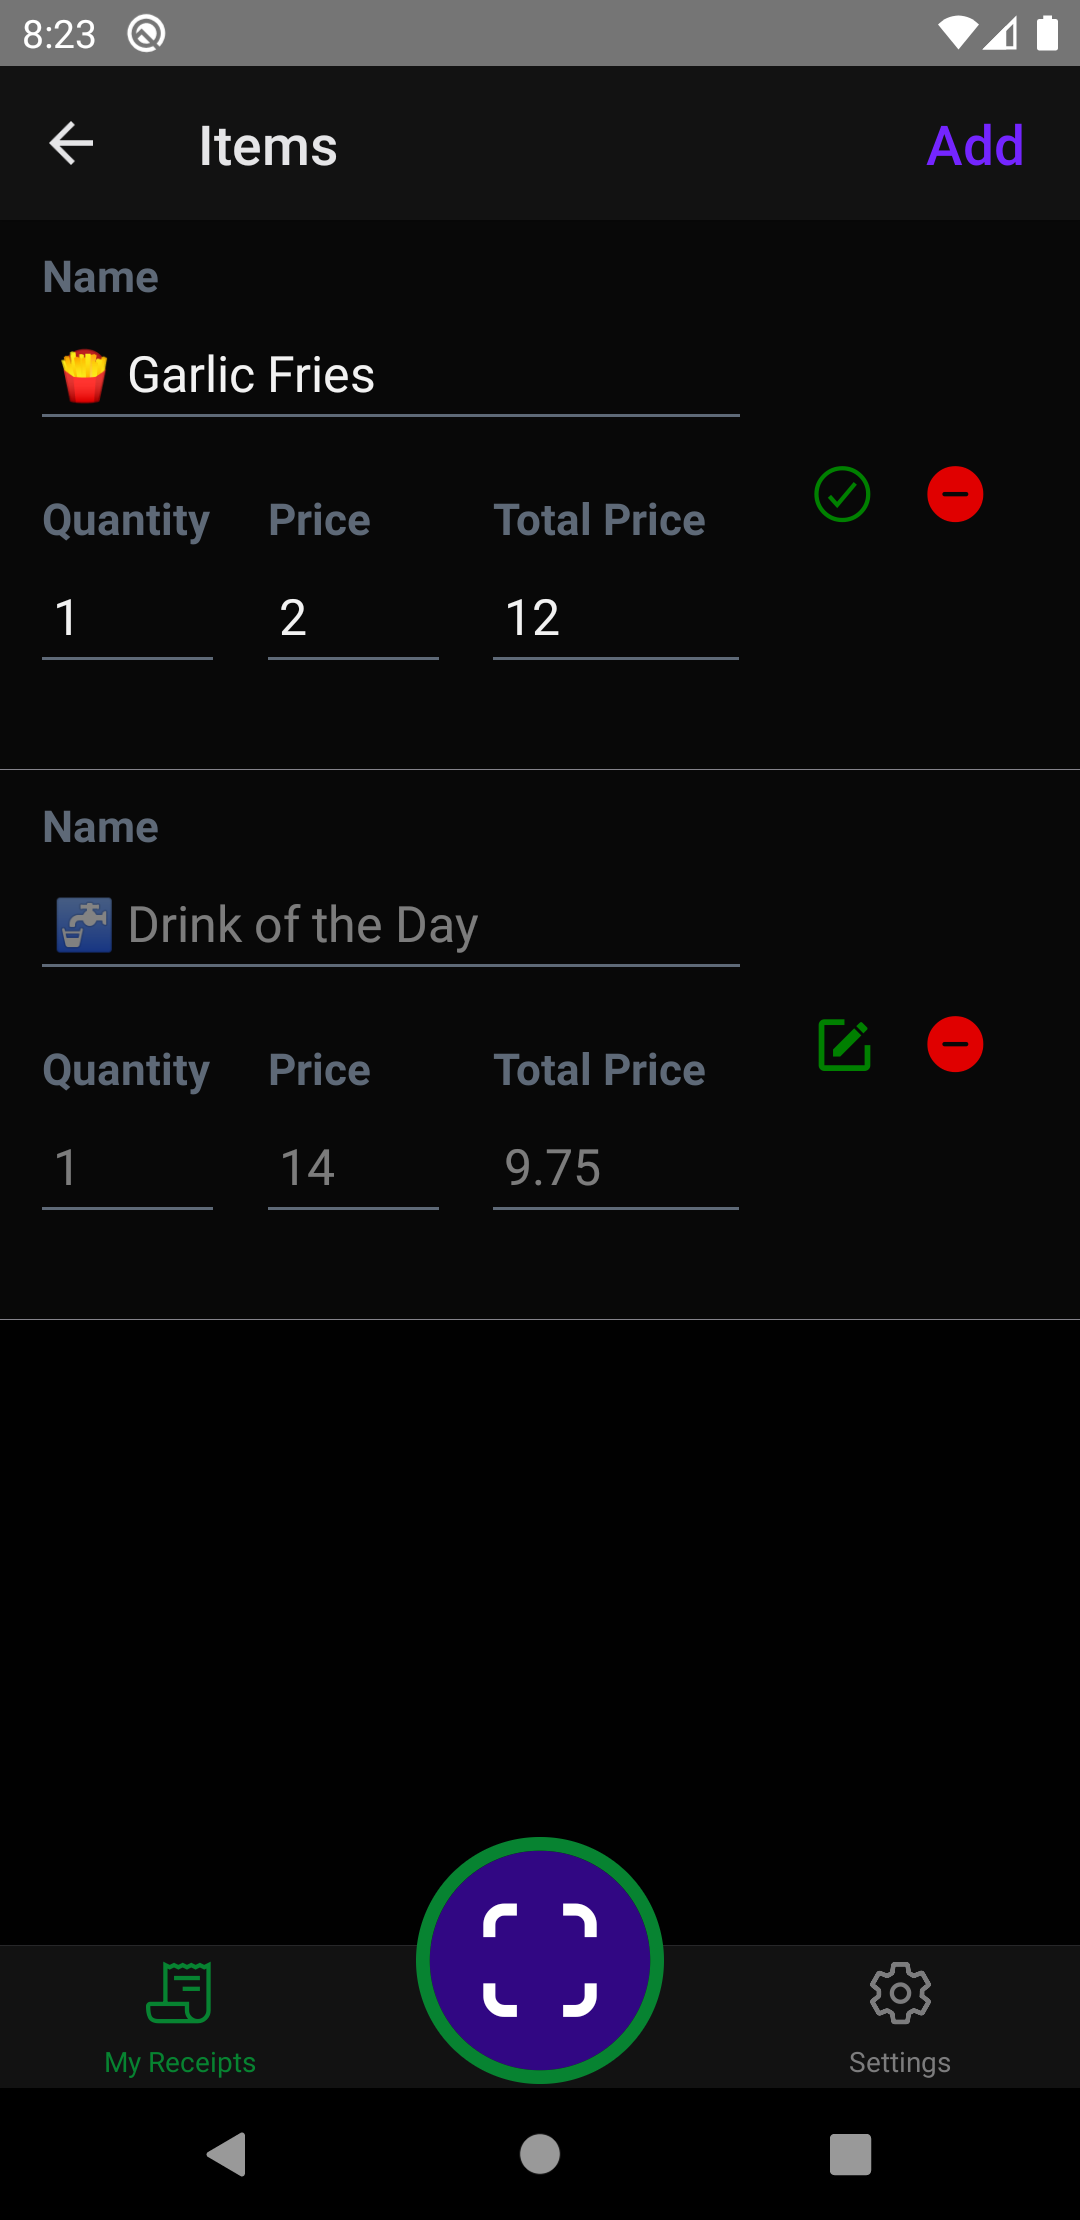
\includegraphics[width=\subfigsize\textwidth]{figures/screens/android/dark/items}
      \caption{A screen with individual receipt items.}
    \end{subfigure}
    \caption{User interface of Receipts Scanner on Android with enabled dark mode.}
    \label{fig:dark_mode_android}
\end{figure}

\begin{figure}
    \centering
    \begin{subfigure}[t]{\half\textwidth}
      \centering
      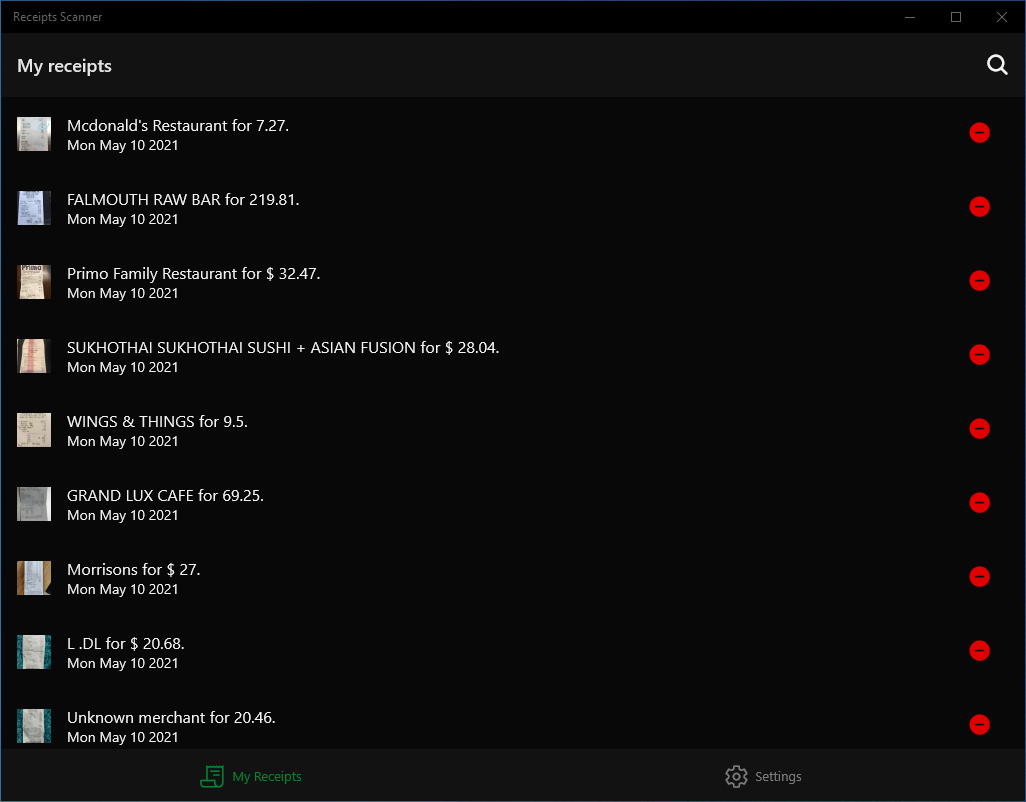
\includegraphics[width=\subfigsize\textwidth]{figures/screens/windows/dark/receipts_list}
      \caption{Main application screen showing list of receipts.}
    \end{subfigure}
    \begin{subfigure}[t]{\half\textwidth}
      \centering
      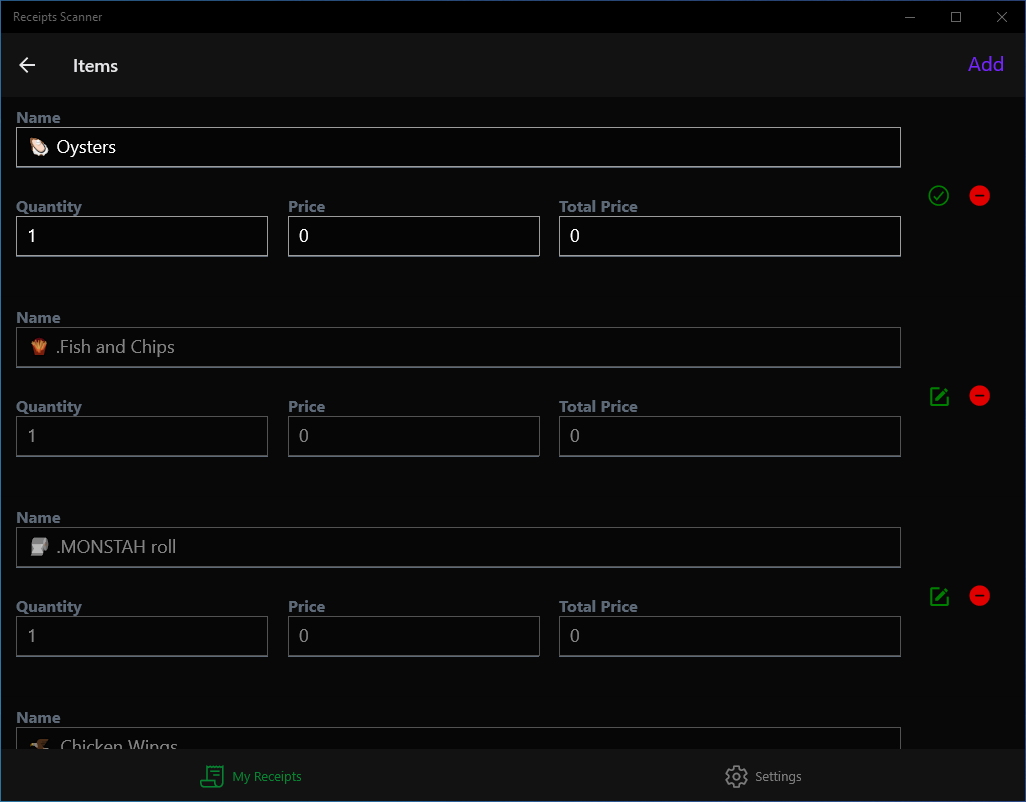
\includegraphics[width=\subfigsize\textwidth]{figures/screens/windows/dark/items}
      \caption{A screen with individual receipt items.}
      \label{fig:dark_mode_windows}
    \end{subfigure}
    \caption{User interface of Receipts Scanner on Windows with enabled dark mode.}
\end{figure}

\section{Real-time user interface}
The receipts are always up to date. Any change in the receipt database for a given user is almost instantly reflected on all other devices where that user is logged in. This means that a user can scan a receipt on the mobile and fill in the receipt information from the PC. If they decide to delete the receipt, the receipt disappears from the other device as well.
This functionality is possible thanks to Google Firebase.

\section{Offline support}
The application works partially offline. Suppose a user is offline and makes any changes to an already existing receipt (edits a receipt, adds a receipt item, deletes a receipt). In that case, the change is reflected in the application UI on the device where the changes were made. Once the user connects to the internet, the changes propagate to the database and other user's devices. The offline changes are persisted even if the application is turned off. This functionality is provided by the Google Firebase library.

The receipt scanning functionality is not possible in an offline mode. If a user tries to scan a receipt without an internet connection, an alert modal window is shown to them.

Ideally, the image would be stored locally, and its thumbnail would be shown among other receipts with a status of \textit{being processed}. After the device connected to the internet again, the image would be sent to Form Recognizer, which would return the extracted data, and the user could complete the pre-filled form.

Another approach would be to use a local model instead of Form Recognizer that would extract the receipt data. This way, the user could complete the complete journey of adding a receipt at once, and the receipt data and the image would be sent to the APIs later on.

Microsoft Form Recognizer does not provide an option to export the model, even if it was a custom one. Therefore a different OCR and data extraction approach would be needed. Furthermore, if the offline model was too large, it should be an opt-in feature of Receipts Scanner.

\section{Features}
This section provides an overview of the functionality available in the Receipts Scanner. Unless stated differently, the feature is available on both platforms, i.e. Android and Windows.

\begin{itemize}
    \item Authentication
        \begin{itemize}
            \item Sign-in/registration with email
            \item Sign-in/registration with Google \Dash only on Android
            \item Email format validation
            \item Password length validation
            \item Preview of password in plain text on toggle 
        \end{itemize}
    \item Adding of receipt \Dash only on Android
        \begin{itemize}
            \item Picking the receipt image from gallery
            \item Taking a photo of the receipt
            \item Receipt image cropping and rotation
            \item Automatic data extraction from the photo that pre-fills the form
            \item Automatic insertion of emoji to each receipt item
        \end{itemize}
    \item Receipt preview
        \begin{itemize}
            \item Preview of the original image
            \item Preview of a processed image for better readability
            \item Purchase date, merchant name, merchant address, merchant phone number, total price, subtotal, tax, tip and currency.
            \item List of receipt items with emoji, name, quantity, price and total price.
        \end{itemize}
    \item Receipt editing
        \begin{itemize}
            \item Editing of purchase date, merchant name, merchant address, merchant phone number, total price, subtotal, tax, tip and currency.
            \item Form fields validation
            \item Fluent navigation between form fields and submitting of form using keyboard only
            \item Ability to add, edit and delete a receipt item
        \end{itemize}
    \item Searching through receipts by merchant name, merchant address and individual names of receipt items
    \item Receipt deletion
    \item Dark mode that reflects system settings
    \item Real-time changes
    \item Partial offline support
    \item Internet connectivity notification \Dash mocked on Windows
    \item Export of receipts data and images
    \item Notification toast messages
\end{itemize}

\chapter{Financial sustainability}
The Receipts Scanner uses paid third-party services, namely:
\begin{itemize}
    \item Microsoft Form Recognizer for OCR and data extraction
    
    \item Google Cloud Build, Google Container Registry and Google Cloud Run for the deployment of Python API container
    
    \item Google Firebase for document database and image storage.
\end{itemize}

The Firebase Authentication is free.

It would be necessary to run the application for some time to figure out the usage statistics, such as the average number of receipts a user uploads. Since those statistics are not available yet, I will provide an \textit{estimate} of the operational costs.

Let us assume that the application has \num{1000} active users, where each user makes one scan per day on average.
The price for Microsoft Form Recognizer is \$0.01 per scan \cite{FormRecognizerPricing}. This means the total cost of this service would be $\num{10000}\cdot30\cdot\$0.01 = \$300.00$.

The size of an uploaded image is around 500 KB, the processed image is smaller, around 100 KB large. The price of storing the textual data is negligible compared to other costs and would be lost in the approximations. Cloud Firestore is a very cheap storage \cite{CloudFirestorePricing} and its free tier provides storage for 1 GB, which is about \num{400000} average-sized receipts\footnote{The size of a stored receipt, \num{2500} KB, was computed using the \textit{firestore-size} library available at \url{https://github.com/alekslario/firestore-size}.}.

Whereas the number of scans is linearly proportional to the number of users, the numbers of stored receipts grows quadratically. It can be expressed recurrently as: 
\begin{equation}
    s(t) = \begin{cases}
        s(t-1) + rut & \text{if }t\geq1\\
        0 & \text{otherwise}
    \end{cases}
\end{equation}
or as a function of $t$:
\begin{equation}
\label{eqn:stored_receipts}
s(t) = \frac{ru}{2}t(t + 1)\text{,}
\end{equation}
where $t$ is a point in time (e.g. month), $r$ is the number of receipts per user per chosen time period (in this case month) and $u$ is the number of new users at the end of the chosen time period (i.e. at the end of a month). Since we assume one receipt per user per day, $r = 30$. Assuming \num{1000} new users per month, $u = \num{1000}$. 
Substitution of the values into the equation \ref{eqn:stored_receipts} gives
\begin{equation}
s(t) = \num{15000}t(t + 1)\text{.}
\end{equation}
A graph of this function is shown in Figure \ref{fig:receipts_by_users}.

\begin{figure}
    \begin{center}
        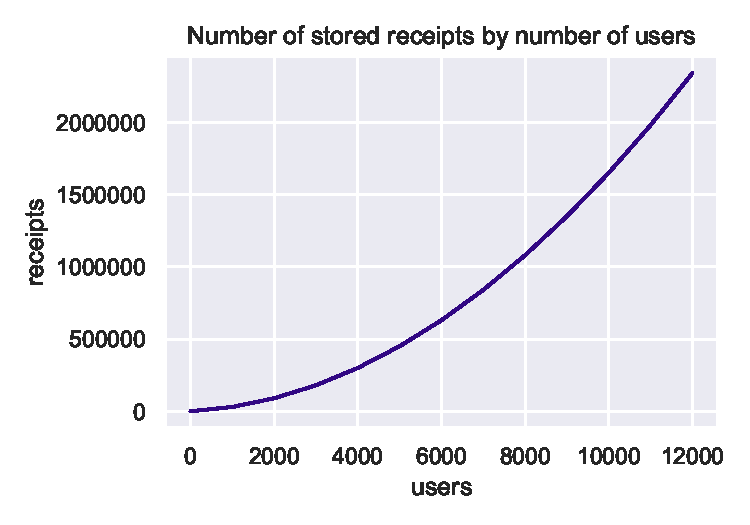
\includegraphics[width=0.7\textwidth]{figures/graphs/receipts_by_users}
    \end{center}
    \caption{Number of stored receipts by number of users}
    \label{fig:receipts_by_users}
\end{figure}

The images of receipts are stored in Google Cloud Storage. The price is \$0.026 per GB \cite{CloudStoragePricing}. For the first month, the cost would be $\num{1000}\cdot30\cdot(600\text{ KB} / 1\text{ GB})\cdot\$0.026 = \$0.468$.
For the second, assuming \num{1000} new users, it would be \$1.404.

The Google Container Registry is charged the same way as Google Cloud Storage \cite{ContainerRegistryPricing}, depending on the size of all stored containers. Even though storing only the newest container would suffice, it is good to keep a few previous containers as well. It is then possible to go back to these containers, should the newest one have any errors. Older containers can be deleted\footnote{Google provides an automated way of deleting old containers available at \url{https://github.com/sethvargo/gcr-cleaner}.}. This means that the price for the stored containers will be fixed. The size of one Python API container is 2.7 GB. The price of storing the five latest containers would be $5\cdot2.7\cdot\$0.02 = \$0.27$ per month. 

Google Cloud Run provides autoscaling, which means that the number of provisioned instances depends on the number of incoming requests. If a minimum number of instances is set to zero, the service goes idle each time the requests are not coming. The service is set up to use 2 CPUs and 6 GB of memory. For each receipt, one request is made to process the image and one to assign categories to items, therefore $\num{1000}\cdot30\cdot2 = \num{60000}$ requests per month. Assuming that each request comes after the previous request ended and that each request takes \num{1000} ms, the service will be used only for \num{120000} vCPU-seconds\footnote{vCPU-seconds are computed as $\textit{number of CPUs} \times \textit{time in seconds the service is running}$.}. This is included in the free plan. Memory consumption would be \num{480000} GiB-seconds\footnote{GiB-seconds are computed as $\textit{size in GiB} \times \textit{time in seconds the service is running}.$}, which slightly exceeds the free plan \cite{CloudRunPricing}, incurring \$0.3 of additional costs. 
If a minimum number of instances was set to one in order to prevent a cold start, the cost would be \$66.00 per month.

Building a container using Google Cloud Build takes approximately 9 minutes. The price is \$0.016 per build-minute \cite{CloudBuildPricing}. Assuming three builds per day due to code changes pushed to the master branch, the cost per month is $3\cdot9\cdot\$0.016\cdot30 = \$12.96$.

The total operational cost per month with \num{1000} users would be \$314.00, i.e. \$0.314 per user.
From Figure 4, it is apparent that most of these costs are due to the OCR service. For this reason, other applications offer the feature of automatic data extraction only after paying a fee. Smart Receipts charges \$0.1 per one OCR scan (as of April 2021).

\begin{figure}
    \begin{center}
        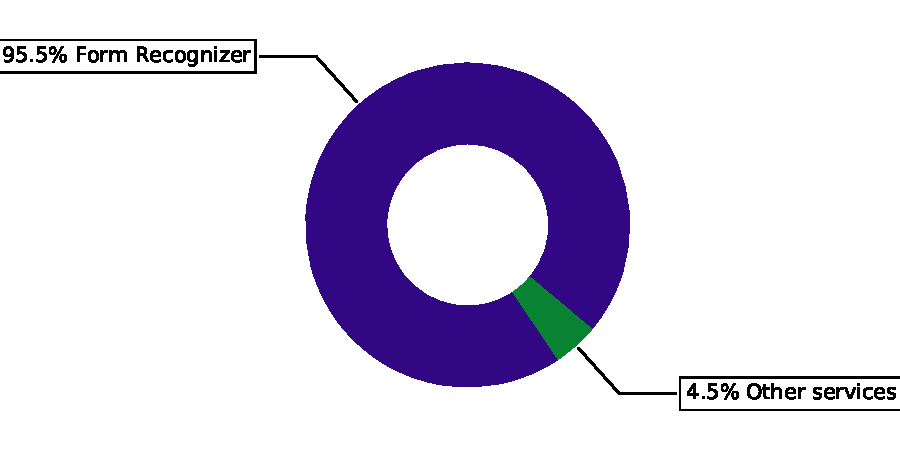
\includegraphics[width=1\textwidth]{figures/graphs/operational_costs}
    \end{center}
    \caption{Operational costs of using Form Recognizer compared to other services}
    \label{fig:operational_costs}
\end{figure}

The Receipts Scanner would therefore need to have its own OCR service or become monetized. In my opinion, in-app advertising, such as AdMob\footnote{Mobile app monetization from Google}, would not generate enough revenue. A subscription-based model seems like a more viable option. The third option would be combining the two previous approaches: a limited number of scans and visible advertisement for non-subscribed users, and an unlimited number of scans and removed advertisement for the subscribed ones.

\chapter{Evaluation}
The application has not been given to real users yet. Therefore there is no available feedback concerning usability, performance and the overall user experience.

The Form Recognizer API used for OCR and data extraction from an image is a third-party service, and as such, measuring its performance would provide little value compared to the rest of the thesis. It would become more important if the current data extraction was insufficient, which would be best found by users in practice.

Quantifying how well Form Recognizer extracts the data from the photo would require a labelled set of receipts. One such set is available as part of the ICDAR2019 Competition on Scanned Receipt OCR
and Information Extraction \cite{Huang2019ICDAR}. It provides \num{1000} labelled receipt scans\footnote{A corrected set of the original images is available on GitHub: \url{https://github.com/zzzDavid/ICDAR-2019-SROIE}.} as well as an evaluation technique. However, the labels from this dataset contain only \textit{company}, \textit{date}, \textit{address} and \textit{total}. Form Recognizer can recognize other information, such as phone number and individual items, too. Furthermore, the main use case in Receipts Scanner is recognition of photographed receipts, not receipt scans. Therefore a different dataset would be needed.

A questionnaire was given to 28 people. It consisted of two parts: evaluation of automatically assigned emojis and comparison of the processed image to the original image regarding readability.

\section{Emoji assignment}
This section aims to evaluate how accurately the emoji chosen by the categorization service inside Python API fits the text. The text is the name of a receipt item recognized by Form Recognizer, consisting of one or more words.

Receipts contain very often abbreviations and names of brands. The categorization service cannot handle those items in a meaningful manner. The assigned emojis in this case are rather arbitrary. An example to illustrate this is \textit{P/DY VEGAN STRAW PROT TUB 1KG} classified as \textit{\emoji{teddy-bear} teddy bear} or \textit{DR PEPPER ZERO} classified as \textit{\emoji{key} key}. TODO Another difficult area is restaurant receipts, which often contain peculiar names of dishes.

Seventy items\footnote{All items from the survey are inserted in the archive in the Information System of Masaryk University \ref{appendix:questionnaire_materials}.} have been selected from the data extracted by Form Recognizer on various receipts, excluding items incorrectly classified as a receipt item and items with which the respondents would be unfamiliar. Duplicates and similar items have not been included in this set either.

For each item and its assigned emoji, the task was to choose whether the emoji is \textit{Not accurate}, \textit{Mildly accurate} or \textit{Accurate}.

As can be seen in Figure \ref{fig:quality_of_emojis}, in the majority of cases, i.e. 53.8\%, the chosen emoji was not accurate. Only in 20.8\% of cases was the emoji considered accurate.

This feature of Receipts Scanner is meant to bring an element of fun into the application, and as such, its functionality is not critical. 

\begin{figure}
    \begin{center}
        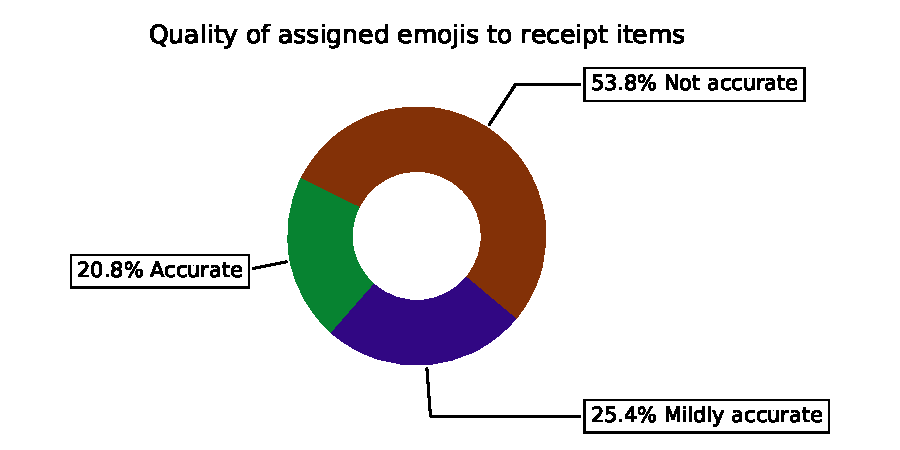
\includegraphics[width=0.7\textwidth]{figures/graphs/quality_of_emojis}
    \end{center}
    \caption{Results of survey evaluating appropriateness of emojis assigned to the receipt items.}
    \label{fig:quality_of_emojis}
\end{figure}

\section{Image processing}
The purpose of this section is to evaluate whether the processed images provide any benefits over the original images.

Thirty receipt photos have been processed using Receipts Scanner. The original and processed images have been placed side by side\footnote{All images from the survey are inserted into the archive in the Information System of Masaryk University \ref{appendix:questionnaire_materials}.}. The task was to choose which image was more readable. As presented in Figure \ref{fig:which_image_is_more_readable}, respondents found 54.5\% of the processed images more readable than the original image.

Sixteen receipts were from the ExpressExpense \cite{ExpressExpense2019Receipt} dataset, and fourteen were taken with modern phone cameras for the purpose of this survey.
All new images and one image from the ExpressExpense dataset were considered more readable in the processed form by most respondents. Two ExpressExpense images had an equal number of votes for each option. The common feature of ExpressExpense receipts is that they have lower quality than the newly taken photos. These results show that the image processing provides a more readable form of the original image if the original image is of sufficiently good quality.

Therefore, the image processing feature of Receipts Scanner will definitely provide value to users, as most modern smartphones can take images of high quality. For the individual cases when the image processing produces worse or even unreadable images, the original image is still available to the users.

\begin{figure}
    \begin{center}
        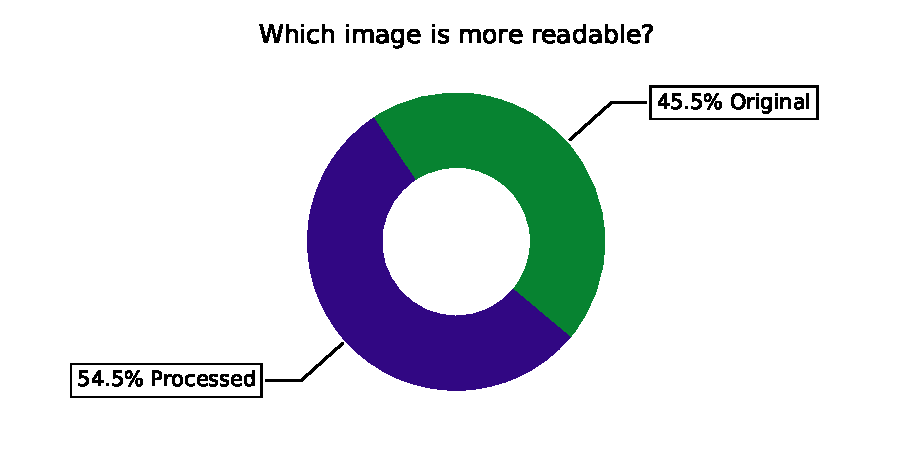
\includegraphics[width=0.7\textwidth]{figures/graphs/which_image_is_more_readable}
    \end{center}
    \caption{Results of survey comparing original and processed images.}
    \label{fig:which_image_is_more_readable}
\end{figure}

\chapter{Conclusion}
lokalizace - form recognizer works only with english receipts, would need to use different solution
explicitne zminit, ze jsem splnil zadani 


% INDEX
\makeatletter\thesis@blocks@clear\makeatother
\phantomsection %% Print the index and insert it into the
\addcontentsline{toc}{chapter}{\indexname} %% table of contents.
\printindex

\appendix %% Start the appendices.

\chapter{Appendix}
\section{Attachments}
Files inserted into the archive in the Information System of Masaryk
University:
\begin{itemize}
% TODO actually add those items
\item receipts\_scanner.zip \Dash Source code of the application.
\item thesis.pdf \Dash Text of the thesis in PDF.
\item questionnaire\_materials.zip \Dash Receipt items and images that have been used in the evaluation survey.
\label{appendix:questionnaire_materials}
\item screenshots.zip \Dash Screenshots of Receipts Scanner on Android/Windows in light/dark mode.
\item receipts\_scanner.apk \Dash Android application package for installation of Receipts Scanner.
\end{itemize}

The latest application source code can be found on GitHub:
\begin{itemize}
\item \url{https://github.com/petr7555/bachelors_thesis_accounting_ocr}
\end{itemize}

\section{Version control system commit messages}

\begin{figure}
    \begin{center}
        \includegraphics[width=\textwidth]{figures/other/Emoji_commits}
    \end{center}
    \caption{Meaning of emojis in commit messages.}
    \label{fig:emoji_commits}
\end{figure}

\end{document}
